\documentclass{beamer}

\usepackage[utf8x]{inputenc}
\usepackage{graphicx}
\usepackage{amsthm,amssymb,amsbsy,amsmath,amsfonts,amssymb,amscd}
\usepackage{dsfont}
\usepackage{tikz}
\usepackage{array}
\newcolumntype{N}{@{}m{2pt}@{}}
\useoutertheme[subsection=false]{miniframes}
\usepackage{lmodern}

\setbeamercolor{author in head/foot}{fg=gray,bg=white}
\setbeamercolor{title in head/foot}{fg=gray,bg=white}
\setbeamercolor{page number in head/foot}{fg=gray,bg=white}
\setbeamercolor{section in head/foot}{bg=black,fg=gray}
\setbeamercolor{subsection in head/foot}{bg=black,fg=gray}

%%%%%%%%%%%%%%%%%%%%%%%%
% GENERAL BEAMER STYLE :

\setbeamertemplate{footline}{
  \hbox{%
    \begin{beamercolorbox}[wd=.2\paperwidth,ht=2ex,dp=1ex,left]{author in head/foot}%
      \hskip1em\usebeamerfont{author in head/foot}\insertshortauthor
    \end{beamercolorbox}%
    \begin{beamercolorbox}[wd=.7\paperwidth,ht=2ex,dp=1ex,center]{title in head/foot}%
      \usebeamerfont{title in head/foot}\insertshorttitle
    \end{beamercolorbox}%
    \begin{beamercolorbox}[wd=.1\paperwidth,ht=2ex,dp=1ex,right]{page number in head/foot}%
      \usebeamerfont{page number in head/foot}\insertframenumber{} / \inserttotalframenumber
      \kern1em 
    \end{beamercolorbox}
  }
}

\setbeamercolor{alerted text}{fg=red!80!black}
\setbeamercolor{itemize/enumerate subbody}{fg=gray!70!black}
\setbeamertemplate{itemize item}[square]
\setbeamertemplate{itemize subitem}[triangle]%{{\textendash}}
\setbeamerfont{itemize/enumerate subbody}{size=\footnotesize}
\setbeamerfont{itemize/enumerate subitem}{size=\footnotesize}

\setbeamertemplate{navigation symbols}{}

\AtBeginSection{
\begin{frame}
    \begin{centering}
    \begin{beamercolorbox}[sep=12pt,center]{part title}
    \usebeamerfont{section title}\insertsection\par
    \end{beamercolorbox}
    \end{centering}
\end{frame}
}

 

%\title[Short course on Statistical Modelling for Optimization -- lecture 1/4]{ \small Short course Statistical Modelling for Optimization -- lecture 1/4 \\ \vspace{3mm} \LARGE Statistical models in engineering}
%\institute[Mines St-\'Etienne]{Nicolas Durrande (durrande@emse.fr) \\ Jean-Charles Croix (jean-charles.croix@emse.fr) \\ Mines St-\'Etienne -- France}
%\author[Pereira, June 2017]{June 2017 -- Universidad Tecnol\'ogica de Pereira -- Colombia}
\title[\'Ecole chercheurs MEXICO]{ \small \'Ecole chercheurs MEXICO, La Rochelle, Mars 2018\\ \vspace{3mm} \LARGE Model Based Optimization}
\author[\quad La Rochelle, March 2018]{Victor Picheny, victor.picheny@inra.fr, Nicolas Durrande, nicolas@prowler.io}
\date{\null}

\DeclareMathOperator*{\Var}{var}
\DeclareMathOperator*{\E}{E}
\DeclareMathOperator*{\Cov}{cov}
\newcommand\PR[1]{\mathrm{P}\left(#1 \right)}
\newcommand\PS[1]{{\langle #1 \rangle}_\mathcal{H}}
\newcommand\PSi[2]{{ \left \langle #1 \right \rangle}_{\! #2}}
\newcommand\N[1]{{|| #1 ||}_\mathcal{H}}
\newcommand\Ni[2]{{|| #1 ||}_{\! #2}}
\newcommand\dx{\, \mathrm{d}}
\newcommand\textequal{\rule[.4ex]{4pt}{0.4pt}\llap{\rule[.7ex]{4pt}{0.4pt}}}
\newcommand{\argmin}{\operatornamewithlimits{argmin}}
\makeatletter
\newcommand{\shorteq}{%
  \settowidth{\@tempdima}{a}% Width of hyphen
  \resizebox{\@tempdima}{\height}{=}%
}
\makeatother
\newcommand\gp{Y}
\newcommand\obs{F}

\definecolor{Orange}{rgb}{0.8, 0.147, 0.0}
\definecolor{MonBleu}{rgb}{0.212, 0.392, 0.545}
%%%%%%%%%%%%%%%%%%%%%%%%%%%%%%%%%%%%%%%%%%%%%%%%%%%%%%
%%%%%%%%%%%%%%%%%%%%%%%%%%%%%%%%%%%%%%%%%%%%%%%%%%%%%%
%%%%%%%%%%%%%%%%%%%%%%%%%%%%%%%%%%%%%%%%%%%%%%%%%%%%%%
\begin{document}

%%%%%%%%%%%%%%%%%%%%%%%%%%%%%%%%%%%%%%%%%%%%%%%%%%%%%%
\begin{frame}
  \titlepage
\end{frame}


%%%%%%%%%%%%%%%%%%%%%%%%%%%%%%%%%%%%%%%%%%%%%%%%%%%%%%%%%%%%%%%%%%%%%%%%%%%%%%%%%%%%
%%%%%%%%%%%%%%%%%%%%%%%%%%%%%%%%%%%%%%%%%%%%%%%%%%%%%%%%%%%%%%%%%%%%%%%%%%%%%%%%%%%%
\section[Global optim.]{Introduction : global optimization}
% \subsection{}

\begin{frame}{}
\begin{block}{Optimisation pour l'aide à la conception / décision}
 \begin{itemize}
  \item Réponse du modèle = performance ou coût
  \item Recherche des paramètres optimaux :
  $$x^* = \arg \min cout(x) \text{ ou } \arg \max {perf(x)}$$
   \end{itemize}
\end{block}

\begin{exampleblock}{Optimisation pour la calibration}
 \begin{itemize}
  \item Sorties du modèle $\Rightarrow$ comparaison à des observations
  \item On veut minimiser un écart quadratique (ou autre métrique)
  $$x^* = \arg \min WLS(x)$$
  \end{itemize}
\end{exampleblock}

\begin{alertblock}{Dans les 2 cas}
 \begin{itemize}
  \item L'optimisation nécessite beaucoup d'appels au code
  \item Métamodèle : solution naturelle
 \end{itemize}
\end{alertblock}

\end{frame}
%-----------------------------------------------------
\begin{frame}
  \frametitle{Le compromis \textbf{exploration / intensification}}
  
  
  \begin{block}{Est-ce qu'on souhaite}
  \begin{itemize}
   \item améliorer une solution existante ?
   \item essayer ``toutes'' les valeurs possibles de paramètres pour trouver la meilleure
  \end{itemize}
 \end{block}

  \begin{block}{Dans la vraie vie : tout essayer n'est pas possible}
  On va chercher un compromis entre 
  \begin{itemize}
   \item améliorer l'existant par de petites modifications
   \item chercher une meilleure solution radicalement différente
  \end{itemize}
  \end{block}
  
\end{frame}
%-----------------------------------------------------
\begin{frame}
  \frametitle{Le compromis \textbf{exploration / intensification}}
  \begin{block}{Optimisation locale}
Amélioration depuis un point initial
  \end{block}

  \begin{block}{Optimisation globale : on cherche un compromis entre}
  \begin{itemize}
   \item Exploration : recherche partout dans l'espace pour ne pas rater la zone optimale 
   \item Intensification : une fois une zone identifiée : on recherche le minimum local
  \end{itemize}
  \end{block}
  
\begin{exampleblock}{Dans un contexte de planification d'expériences}
  \begin{itemize}
   \item Exploration : remplissage d'espace
   \item Intensification : ``ciblage''
  \end{itemize}
\end{exampleblock}
  
\end{frame}
%-----------------------------------------------------
\begin{frame}
  \frametitle{Introduction à l'optimisation globale : l'algorithme DIRECT}
  Garanti sans métamodèle !
  \begin{block}{DIRECT : DIviding RECTangles}
  \begin{itemize}
   \item Découpage de l'espace en (hyper)rectangles
   \item Un échantillon au centre de chaque rectangle
   \item On divise les rectangles les plus ``intéressants'' :
   \begin{itemize}
     \item soit les plus grands (exploration)
     \item soit ceux qui ont une valeur au centre basse (intensification)
   \end{itemize}
   \item Pour diviser : ajout de 2 points, division en 3
  \end{itemize}
  \end{block}
  \scriptsize{
 \begin{thebibliography}{7}
\beamertemplatearticlebibitems
%\beamertemplatebookbibitems
     \bibitem{direct}
     D.~Jones, C.~Perttunen, B.~Stuckman (1993)
         \newblock Lipschitzian optimization without the Lipschitz constant
         \newblock Journal of Optimization Theory and Applications 79(1), 157-181
 \end{thebibliography}
}
\normalsize
%   \begin{block}{Compromis exploration / intensification}
% Pour (presque) \textbf{chaque} taille de rectangle, on divise celui qui a la meilleure valeur observée
%   \end{block}
%   
\end{frame}
%-----------------------------------------------------
\begin{frame}
\frametitle{Exemple en dimension 2}
%   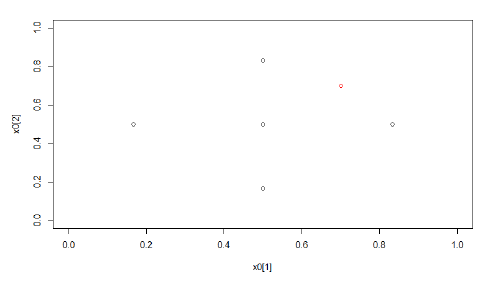
\includegraphics[width=.45\paperwidth]{fig/direct1.png}
%   \\
\begin{itemize}
 \item Départ : 3 points équirépartis dans une direction aléatoire
 \item On divise le rectangle ayant la meilleure observations
\end{itemize}

  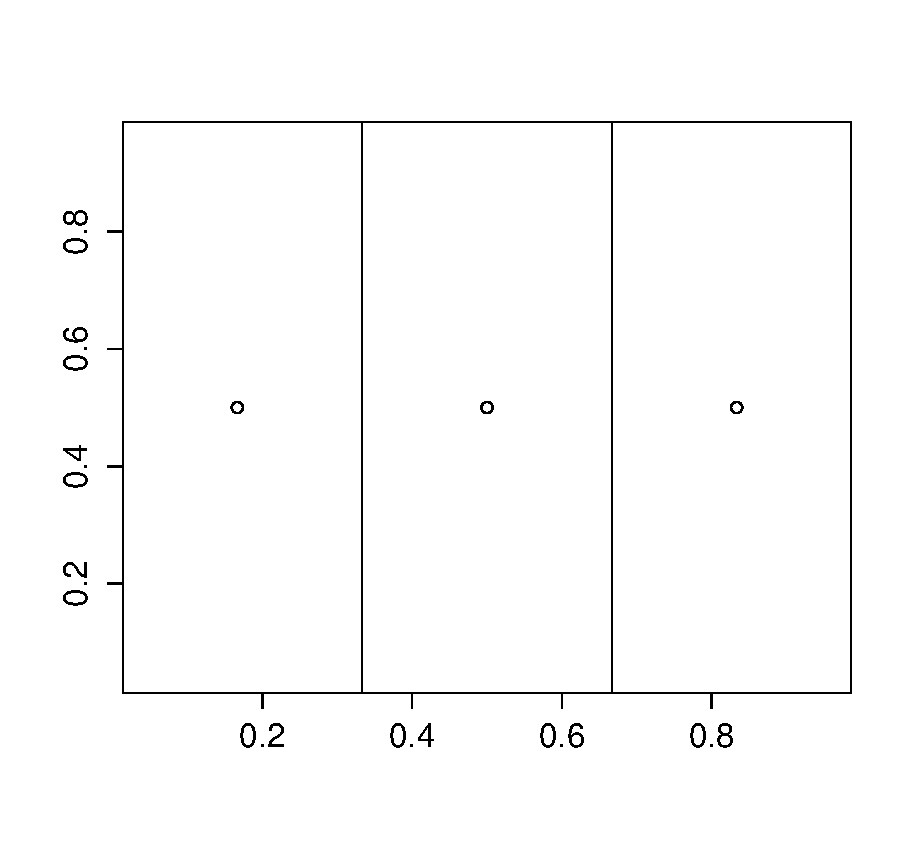
\includegraphics[width=.45\textwidth]{fig/direct1.pdf} \hspace{5mm}
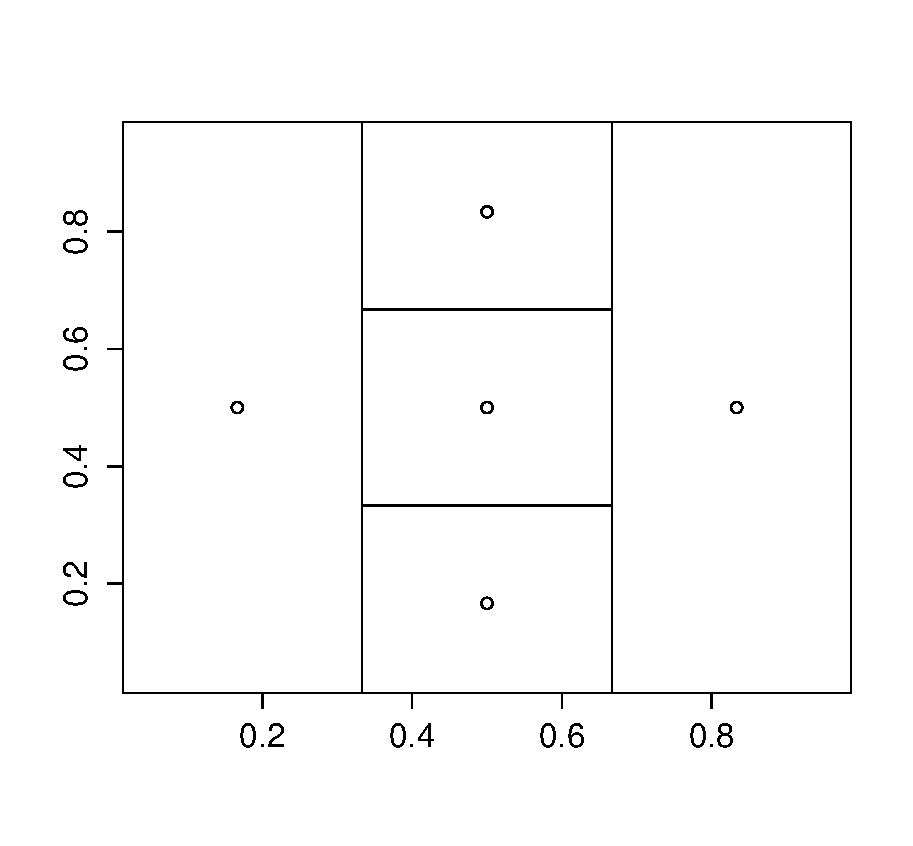
\includegraphics[width=.45\textwidth]{fig/direct1bis.pdf}
  \end{frame}

%-----------------------------------------------------
\begin{frame}
\frametitle{Exemple en dimension 2}
%   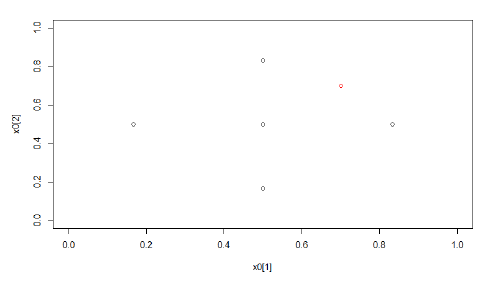
\includegraphics[width=.45\paperwidth]{fig/direct1.png}
%   \\
  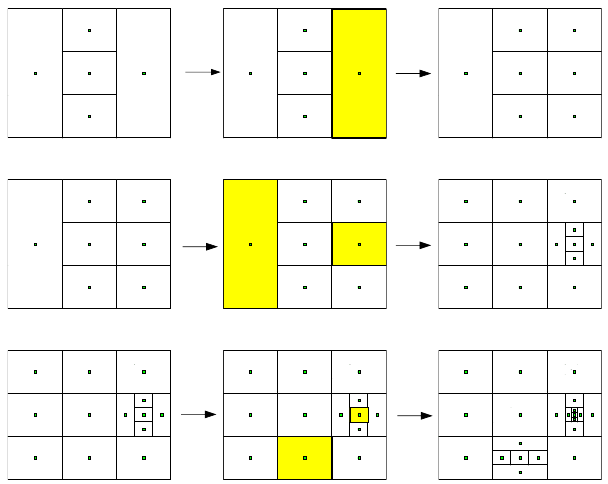
\includegraphics[width=.9\textwidth]{fig/direct2.png}
\end{frame}

%-----------------------------------------------------
\begin{frame}
\frametitle{Après 191 évaluations}
\begin{itemize}
 \item Echantillonnage intense dans la zone de l'optimum
 \item Bonne exploration 
\end{itemize}



\begin{columns}
 \begin{column}{80mm}
 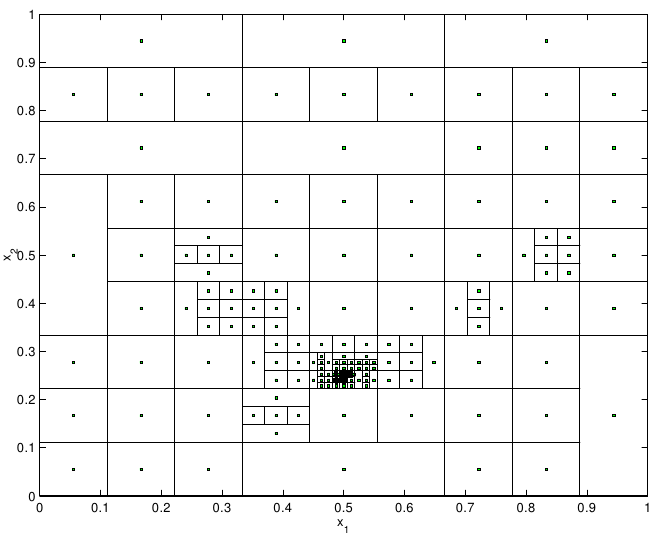
\includegraphics[width=\textwidth]{fig/direct3.png}  
 \end{column}
 \begin{column}{40mm}
   \scriptsize{Source figures :
 \begin{thebibliography}{1}
\beamertemplatearticlebibitems
     \bibitem{fin}
     D. E. Finkel
         \newblock DIRECT Optimization Algorithm User Guide (2003)
 \end{thebibliography}}
 \end{column}
\end{columns}
\end{frame}
%-----------------------------------------------------
\begin{frame}
\frametitle{Intêret et limites}
\begin{itemize}
 \item[$+$] Exploration de tout l'espace de recherche
 \item[$+$] Stratégie robuste
 \item[$-$] Limité aux petites dimensions
 \item[$-$] Exploitation limitée de l'information
\end{itemize}
\vspace{5mm}
$\Rightarrow$ même principe général, avec un métamodèle ?
\end{frame}
%-----------------------------------------------------
\section[Trust regions]{Trust regions (quadratic metamodels)}
%-----------------------------------------------------
%%%%%%%%%%%%%%%%%%%%%%%%%%%%%%%%%%%%%%%%%%%%%%%%%%%%%%
\begin{frame}{}
Si le nombre d'appels au modèle est trop limité, on peut optimiser le métamodèle à la place :

\begin{center}
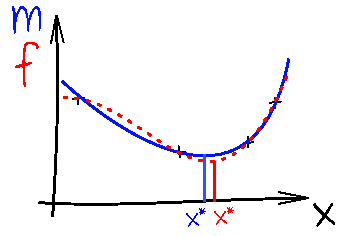
\includegraphics[height=5cm]{figures/ink_mf}
\end{center}
Et on espère qu'à la fin on ait :
\begin{equation*}
	\begin{split}
		\argmin(m) & \approx \argmin(f)\\
		\min(m) & \approx \min(f)\\
	\end{split}
\end{equation*}
\end{frame}

%%%%%%%%%%%%%%%%%%%%%%%%%%%%%%%%%%%%%%%%%%%%%%%%%%%%%%
\begin{frame}{}
\structure{Schéma global}
  \begin{figure}
    \centering \sf
    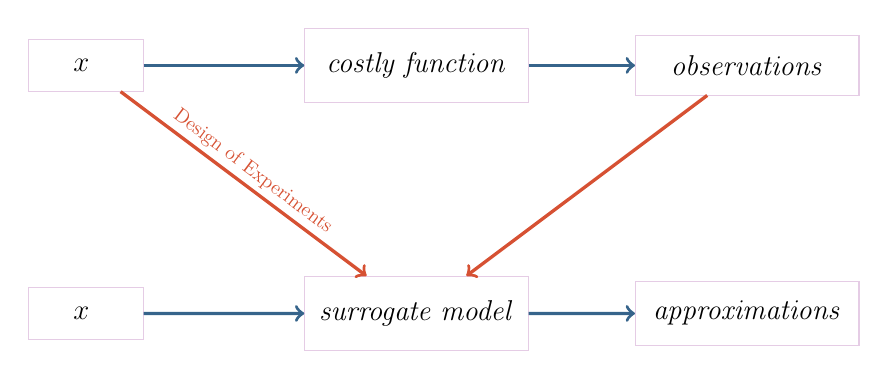
\begin{tikzpicture}[scale=0.7, every node/.style={scale=0.6}]

      % \tikzstyle{Sim}=[rectangle, draw=MonBleu!20, fill=MonBleu!0];
      % \tikzstyle{Meta}=[rectangle, draw=Orange!40, fill=MonBleu!0];
      \tikzstyle{Mes}=[rectangle, draw=violet!20, fill=violet!0];

        \node[Mes](MesIn) at (-6, 0) {
          \parbox{2.2cm}{ %
            \centering
            \LARGE
            \vspace{3mm}
            $x$
            \vspace{3mm}
          }};

        \node[Mes](Mes) at (0, 0) {
          \parbox{4.5cm}{ %
            \centering
            \LARGE
            \vspace{4mm}
            \textit{costly function}\\
            \vspace{4mm}
          }};

        \node[Mes](MesOut) at (6, 0) {
        \parbox{4.5cm}{ %
            \centering
            \LARGE
            \vspace{3mm}
          \textit{observations}\\
            \vspace{3mm}
        }};
        \draw[->, very thick, draw=MonBleu] (MesIn) -- (Mes.west);
        \draw[->, very thick, draw=MonBleu] (Mes) -- (MesOut.west);

        \node[Mes](MetaIn) at (-6, -4.5) {
          \parbox{2.2cm}{ %
          \centering
            \LARGE
            \vspace{3mm}
            $x$
            \vspace{3mm}
          }};

        \node[Mes](Meta) at (0, -4.5) {
          \parbox{4.5cm}{ %
            \centering
            \LARGE
            \vspace{4mm}
            \textit{surrogate model}\\
            \vspace{4mm}
          }};

        \node[Mes](MetaOut) at (6.0, -4.5) {
        \parbox{4.5cm}{ %
            \centering
            \LARGE
            \vspace{3mm}
          \textit{approximations}\\
            \vspace{3mm}
        }};

        \draw[->, very thick, draw=MonBleu] (MetaIn) -- (Meta.west);
        \draw[->, very thick, draw=MonBleu] (Meta) -- (MetaOut.west);

        \draw[->, very thick, draw=Orange!80] (MesIn) -- (Meta)
        node [above, midway, sloped, Orange!80] {\large Design of Experiments};
        \draw[->, very thick, draw=Orange!80] (MesOut)  -- (Meta);
        %node [above, midway, sloped, Orange!80] {\large réponses};

    \end{tikzpicture}
    \end{figure}
\end{frame}

\begin{frame}
\frametitle{Optimisation et métamodèle : ce qu'on est tenté de faire...}
\begin{columns}[c]
 \begin{column}{.51\textwidth}
  
\begin{block}{``Le métamodèle donne l'optimum''}
 \begin{itemize}
  \item On cherche le minimum $x^*$ sur le métamodèle
  \item On évalue le vrai $y(x^*)$ sur le simulateur
 \end{itemize}
$\Rightarrow$ C'est fini !
\end{block}

\begin{block}{Répartition de l'effort}
 \begin{itemize}
  \item Plan initial : 49 expériences
  \item 98\% exploration, 2\% exploitation
 \end{itemize}
\end{block}
 \end{column}
 \begin{column}{.49\textwidth}
  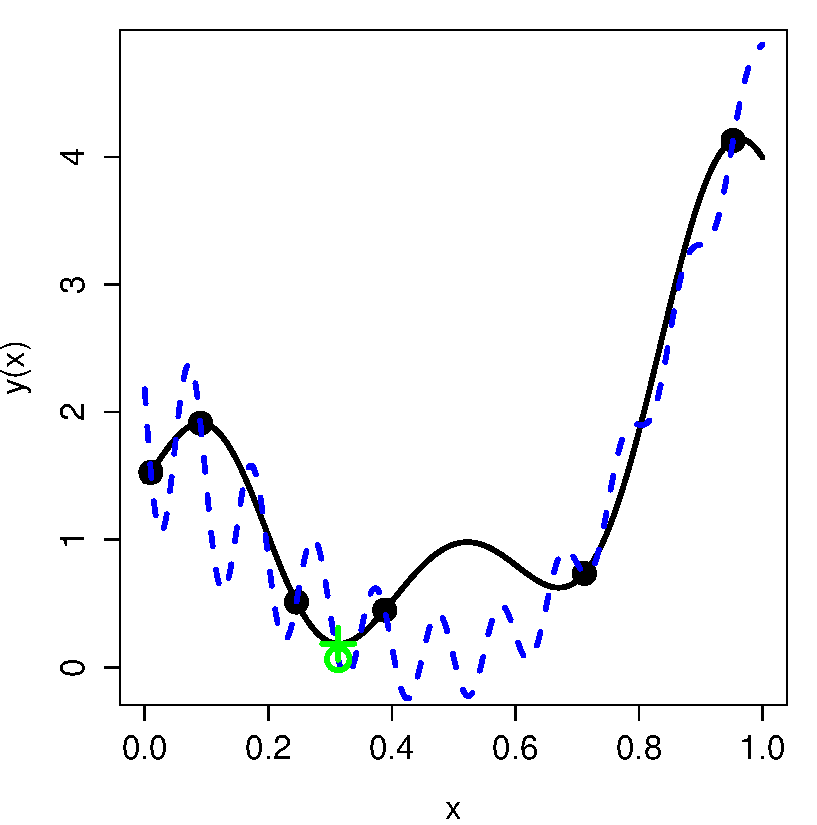
\includegraphics[width=\textwidth]{fig/exoptim1.pdf}
 \end{column}
\end{columns}
\vspace{1mm}
\centering
\alert{Que faire si $x^*$ n'est pas bon ?}
\end{frame}

%-----------------------------------------------------
\begin{frame}
\frametitle{Optimisation et métamodèle : ce qu'il faut faire}
\begin{block}{Si le budget est fixe}
 \begin{itemize}
  \item On divise le budget en 2
  \item Budget 1 : plan initial (LHS)
  \item Budget 2 : optimisation
 \end{itemize}
\end{block}

\begin{block}{Utilisation \textbf{séquentielle} du métamodèle}
 \begin{itemize}
  \item Métamodèle initial : \textit{a priori} peu précis
  \item Le métamodèle sert à \textbf{choisir} pour les nouvelles observations
  \item A chaque nouvelle observation : amélioration du métamodèle
 \end{itemize}
\end{block}
\end{frame}

% -----------------------------------------------------
\begin{frame}
\frametitle{Schéma général : métamodèle = guide}

   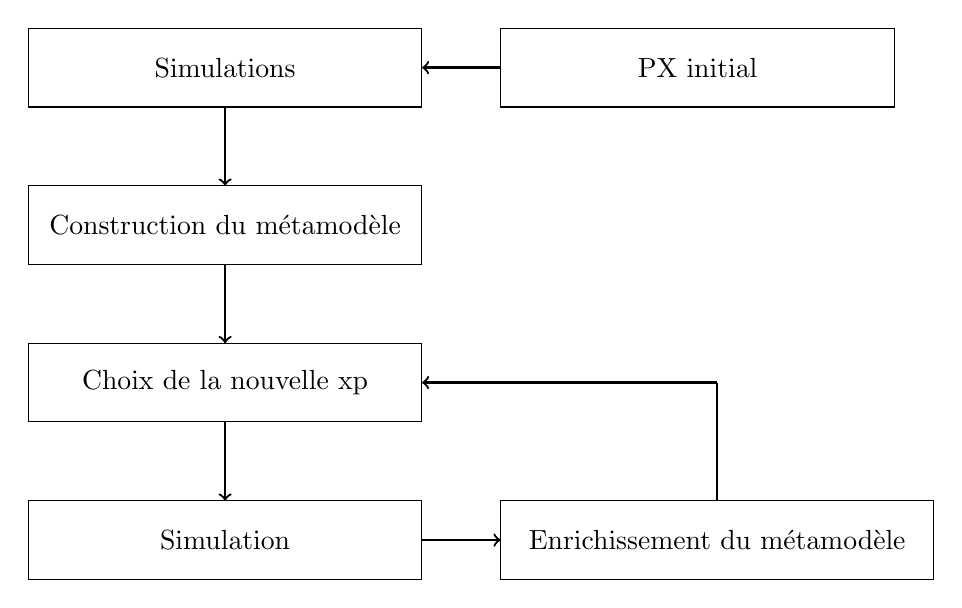
\begin{tikzpicture}[scale=1]
   \draw(6,2) rectangle (11,3);
   \draw(8.5,2.5) node{PX initial};
   
   \draw[<-,thick] (5,2.5)--(6,2.5);
   
   \draw(0,2) rectangle (5,3);
   \draw(2.5,2.5) node{Simulations};
   
   \draw[<-,thick] (2.5,1)--(2.5,2);
   
   \draw(0,0) rectangle (5,1);
   \draw(2.5,.5) node{Construction du métamodèle};
 \draw[<-,thick] (2.5,-1)--(2.5,0);
    \draw(0,-2) rectangle (5,-1);
   \draw(2.5,-1.5) node{Choix de la nouvelle xp};
 \draw[<-,thick] (2.5,-3)--(2.5,-2);
     \draw(0,-4) rectangle (5,-3);
   \draw(2.5,-3.5) node{Simulation};
  
  \draw[->,thick] (5,-3.5)--(6,-3.5);
  
   \draw(6,-4) rectangle (11.5,-3);
   \draw(8.75,-3.5) node{Enrichissement du métamodèle};
  \draw[-,thick] (8.75,-3)--(8.75,-1.5);
  \draw[<-,thick] (5,-1.5)--(8.75,-1.5);
 \end{tikzpicture}
\end{frame}

%-----------------------------------------------------
% \subsection{Optimisation basée sur les modèles polynomiaux}
%-----------------------------------------------------
\begin{frame}
\frametitle{Optimisation basée sur les modèles polynomiaux}
\begin{block}{Principe}
 \begin{itemize}
  \item On construit une surface de réponse $y = \beta_0 + \beta_1 x + \beta_2 x^2$
  \item On cherche le point qui minimise la surface de réponse
  \item On ajoute ce point
  \item On met à jour la surface de réponse
  \item On recommence...
 \end{itemize}
\end{block}

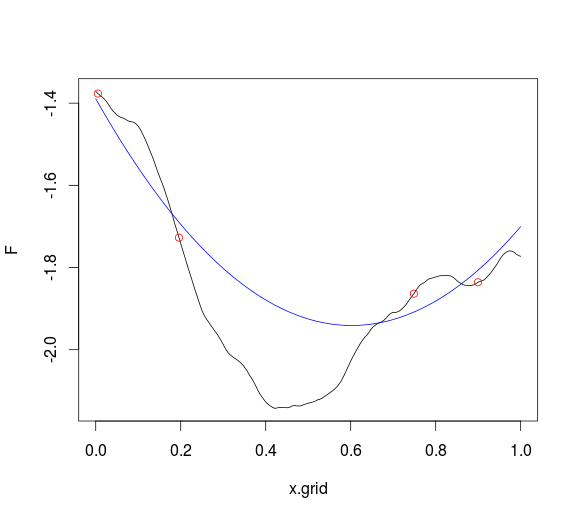
\includegraphics[trim = 10mm 20mm 10mm 10mm, clip, width=.37\paperwidth]{fig/prs1.png}
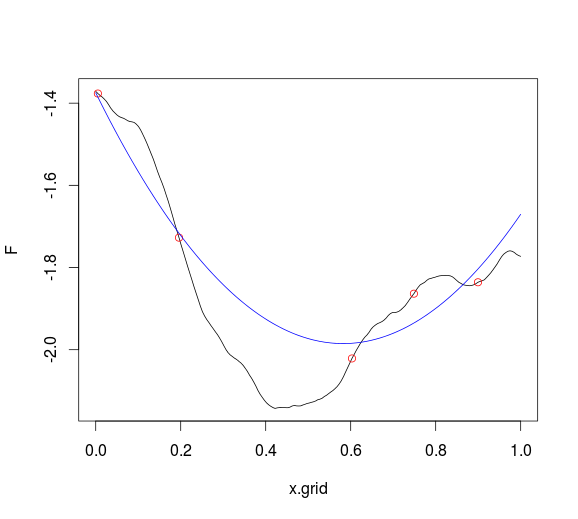
\includegraphics[trim = 10mm 20mm 10mm 10mm, clip, width=.37\paperwidth]{fig/prs2.png}
\end{frame}

%-----------------------------------------------------
%-----------------------------------------------------
\begin{frame}
\frametitle{Itérations 3 à 7}
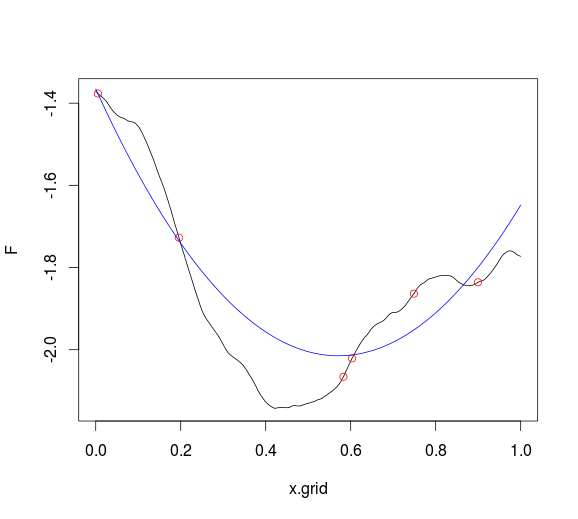
\includegraphics[trim = 10mm 20mm 10mm 10mm, clip, width=.31\textwidth]{fig/prs3.png}
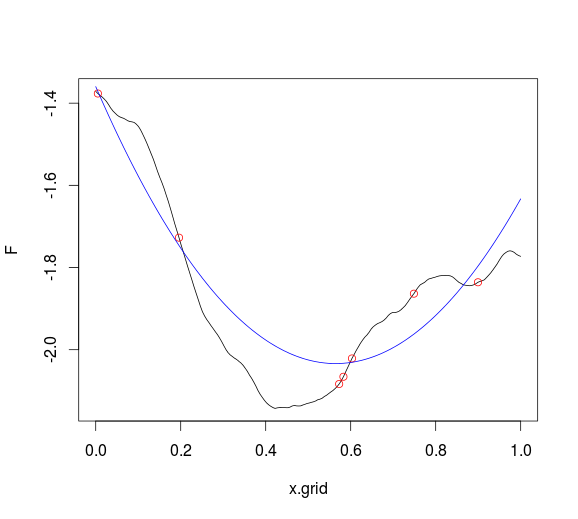
\includegraphics[trim = 10mm 20mm 10mm 10mm, clip, width=.31\textwidth]{fig/prs4.png}
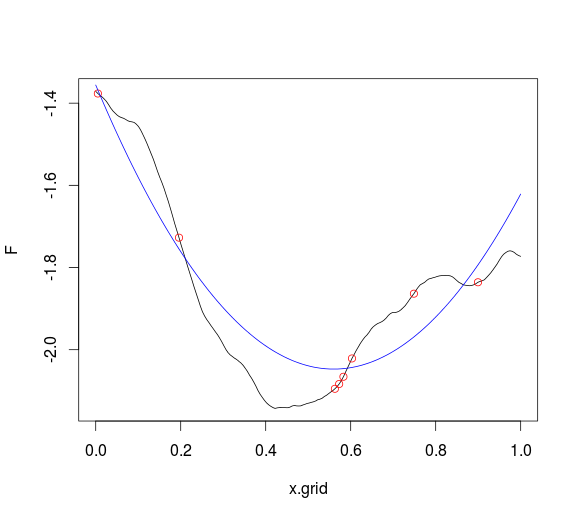
\includegraphics[trim = 10mm 20mm 10mm 10mm, clip, width=.31\textwidth]{fig/prs5.png}
\\
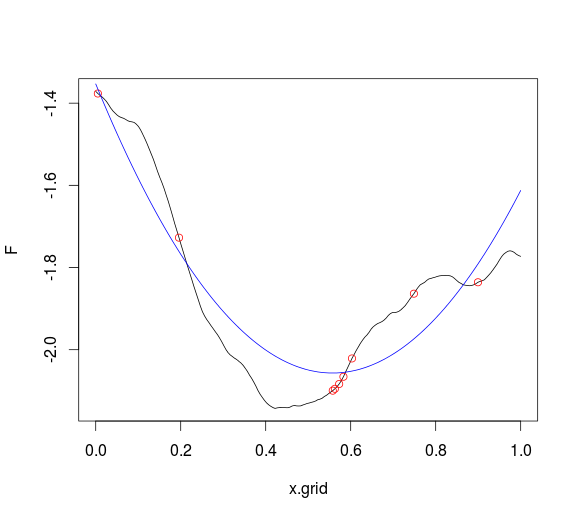
\includegraphics[trim = 10mm 20mm 10mm 10mm, clip, width=.31\textwidth]{fig/prs6.png}
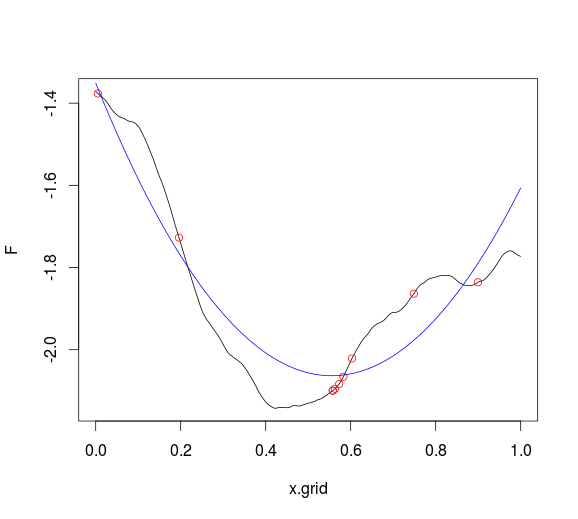
\includegraphics[trim = 10mm 20mm 10mm 10mm, clip, width=.31\textwidth]{fig/prs7.png}
\end{frame}
%-----------------------------------------------------
\begin{frame}
\frametitle{Optimisation basée sur les modèles polynomiaux}
\begin{block}{Problème : modèle ``rigide''}
Le modèle ne s'ajuste pas aux données : 
$ Y = \mathbf{X} \beta + \epsilon $

Pas de convergence vers un modèle précis, même localement
\end{block}

\begin{exampleblock}{Solutions}
\begin{enumerate}
 \item Augmenter le dégré du polynôme \\
 \textcolor{red}{$\Rightarrow$ risque de surapprentissage \& d'instabilité !}
 \item Supprimer des points \\
 $\Rightarrow$ méthode \textbf{de région de confiance}
\end{enumerate}
\end{exampleblock}
\end{frame}

%-----------------------------------------------------
\begin{frame}
\frametitle{Régions de confiance : principe}
\begin{block}{Modèle quadratique ``creux''}
\begin{itemize}
 \item Valide à l'intérieur d'une région de confiance (petite)
 \item Construit uniquement avec les points à l'intérieur de la région
 \item Selon les valeurs des simulations, on modifie la taille de la région
\end{itemize}
\end{block}

\begin{block}{Gestion de la région de confiance}
A chaque itération :
\begin{itemize}
 \item $\hat y (x^*)$ bon $\Rightarrow$ confiance dans le modèle : on augmente la taille
 \item $\hat y (x^*)$ mauvais $\Rightarrow$ modèle peu fiable : on diminue la taille
\end{itemize}
\end{block}
+ beaucoup de règles pour sélectionner les points et enrichir le plan d'expériences
\end{frame}
%-----------------------------------------------------
\begin{frame}
\frametitle{Illustration (source : F. Vanden Berghen)}
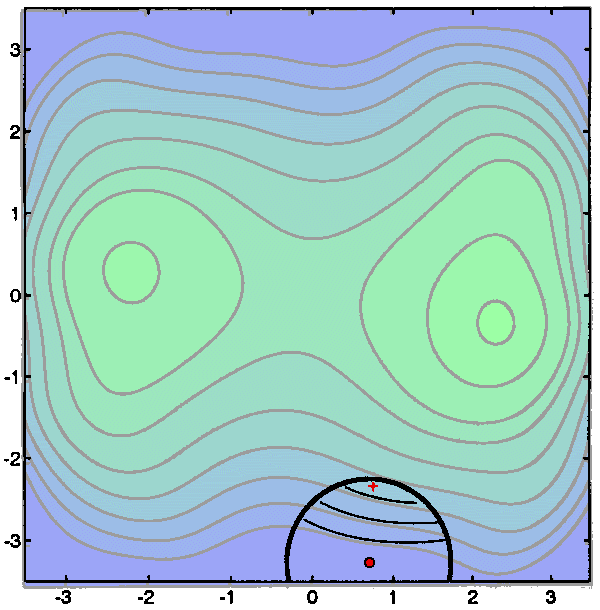
\includegraphics[width=.49\textwidth]{trm/Image2.png}
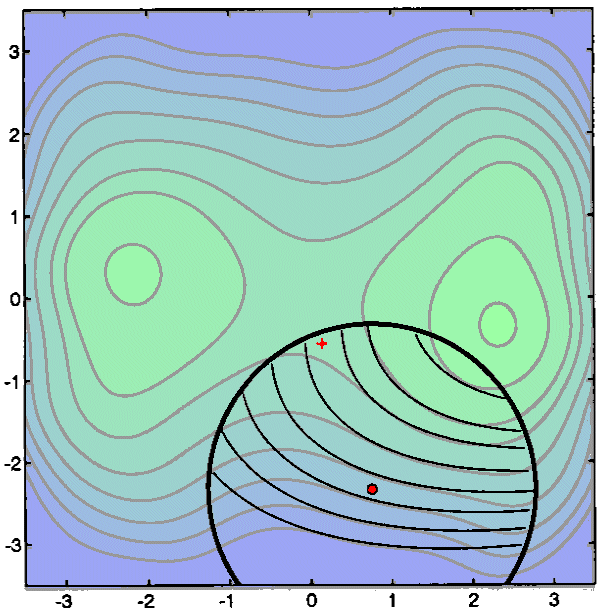
\includegraphics[width=.49\textwidth]{trm/Image3.png}
\end{frame}
%-----------------------------------------------------
\begin{frame}[noframenumbering]
\frametitle{Illustration (source : F. Vanden Berghen)}
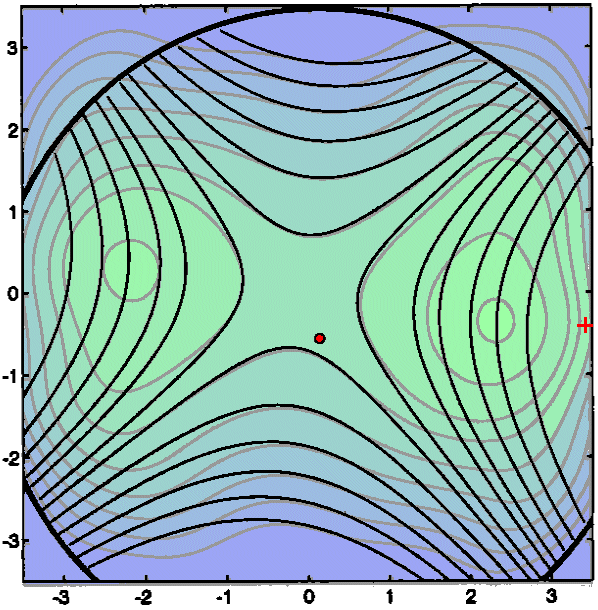
\includegraphics[width=.49\textwidth]{trm/Image4.png}
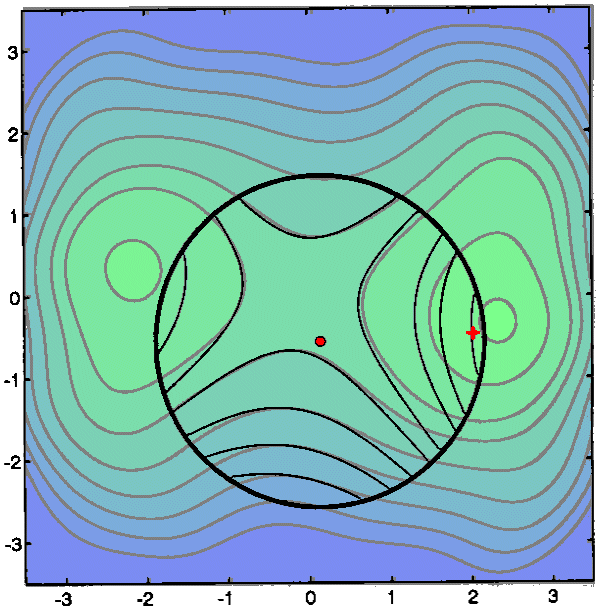
\includegraphics[width=.49\textwidth]{trm/Image5.png}
\end{frame}
%-----------------------------------------------------
\begin{frame}[noframenumbering]
\frametitle{Illustration (source : F. Vanden Berghen)}
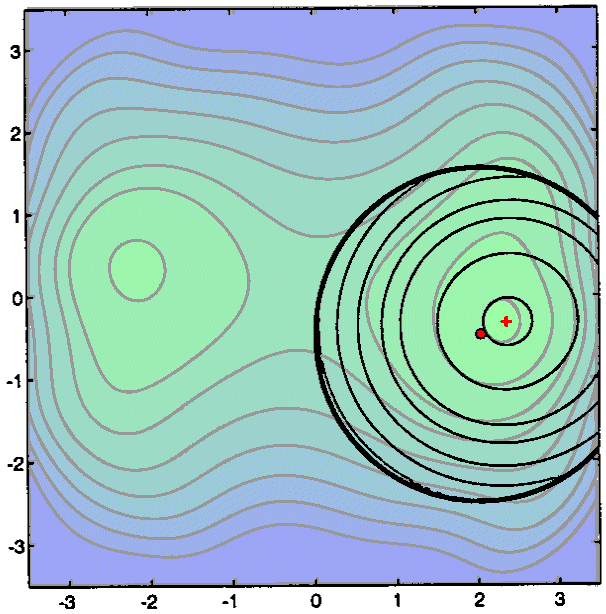
\includegraphics[width=.49\textwidth]{trm/Image6.png}
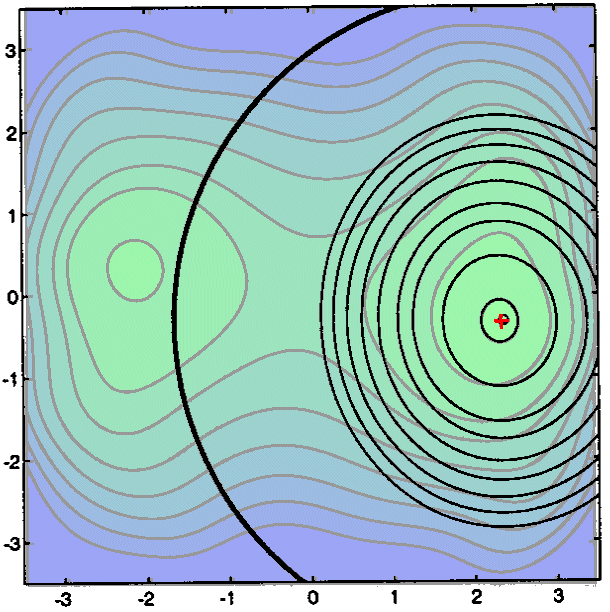
\includegraphics[width=.49\textwidth]{trm/Image7.png}
\end{frame}
%-----------------------------------------------------
\begin{frame}
\frametitle{}
\begin{block}{Avantages}
\begin{itemize}
 \item Garantie de convergence
 \item Méthodes assez parcimonieuses
 \item Robuste
 \item Accepte un très grand nombre de variables
\end{itemize}
\scriptsize{
 \begin{thebibliography}{1}
\beamertemplatearticlebibitems
     \bibitem{conn}
     Conn, Scheinberg, and Vicente
         \newblock Introduction to derivative-free optimization
         \newblock MPS-SIAM Series on Optimization (2009)
          \bibitem{newuoa}
          Powell
         \newblock The NEWUOA software for unconstrained optimization without derivatives
         \newblock Large-scale nonlinear optimization (2006)    
 \end{thebibliography}}
\end{block}

\begin{alertblock}{Méthode locale (proche méthode de gradient)}
Pas de métamodèle final utilisable globalement - mais gradient + hessien !
\end{alertblock}
\end{frame}
%%%%%%%%%%%%%%%%%%%%%%%%%%%%%%%%%%%%%%%%%%%%%%%%%%%%%%
\section[EG0]{Kriging-based optimization (EGO)}
%%%%%%%%%%%%%%%%%%%%%%%%%%%%%%%%%%%%%%%%%%%%%%%%%%%%%%
\begin{frame}{}
\textbf{Global optimization} methods are a trade-off between
\begin{itemize}
	\item Exploitation of past good results
	\item Exploration of the space
\end{itemize}
\vspace{3mm}
\begin{center}
\textbf{How can GPR models be helpful?}\\
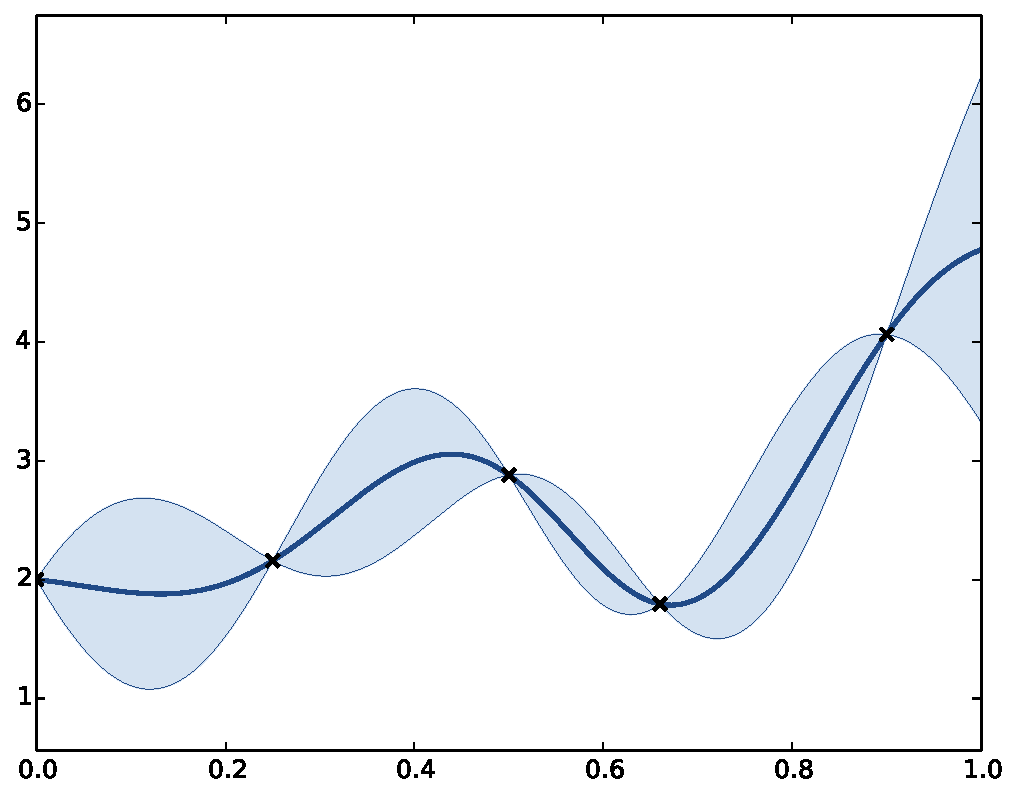
\includegraphics[height=5cm]{figures/python/ego_0}
\end{center}
\end{frame}

%%%%%%%%%%%%%%%%%%%%%%%%%%%%%%%%%%%%%%%%%%%%%%%%%%%%%%
\begin{frame}{}
In our example, the best observed value is 1.79
\begin{center}
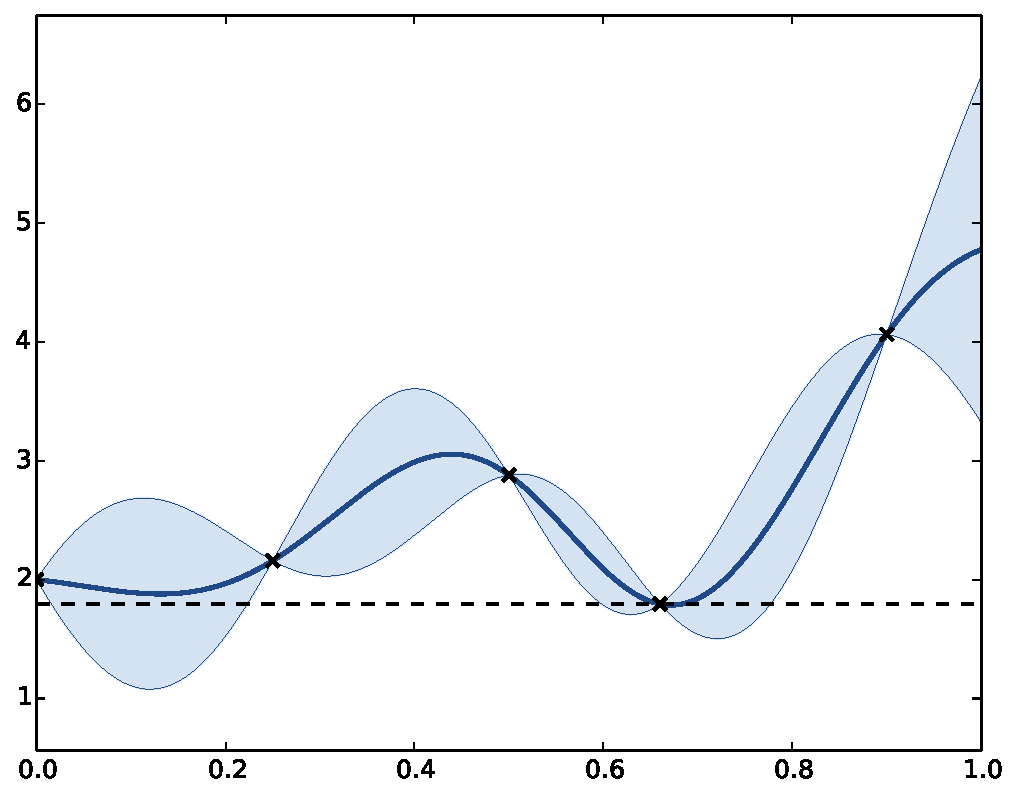
\includegraphics[height=5cm]{figures/python/ego_improv}
\end{center}
Various criteria can be studied
\begin{itemize}
	\item probability of improvement
	\item Expected improvement
\end{itemize}
\end{frame}

%%%%%%%%%%%%%%%%%%%%%%%%%%%%%%%%%%%%%%%%%%%%%%%%%%%%%%
\begin{frame}{}
\textbf{Probability of Improvement:}
$$PI(x) = cdf \left(\frac{\min(F) - m(x)}{\sqrt{(c(x,x))}} \right)$$
\begin{center}
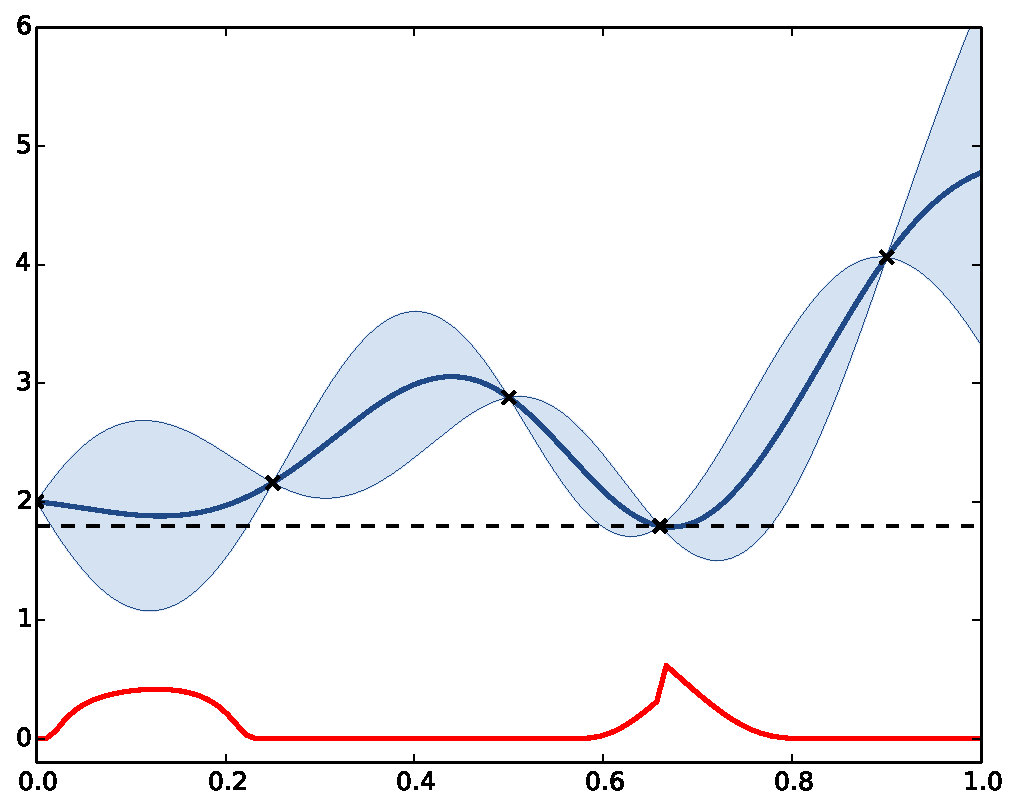
\includegraphics[height=5cm]{figures/python/ego_PI}
\end{center}
\end{frame}

%%%%%%%%%%%%%%%%%%%%%%%%%%%%%%%%%%%%%%%%%%%%%%%%%%%%%%
\begin{frame}{}
The point with the highest PI is often very close to the best observed value. We can show that there is a $x$ in the neighbourhood of $x^*$ such that $PI(x) \geq 0.5$.\\
\vspace{5mm}
For such points, the improvement cannot be large... \\
\vspace{3mm}
Can we find another criterion?
\end{frame}

%%%%%%%%%%%%%%%%%%%%%%%%%%%%%%%%%%%%%%%%%%%%%%%%%%%%%%
\begin{frame}{}
\textbf{Expected Improvement:}
\begin{equation*}
\begin{split}
E&I(x) =  \int_{-\infty}^{\min(F)} \max\left(0,Y(x)\right) ~dy(x) = \dots = \\
& \sqrt{c(x,x)} (u(x) cdf(u(x)) + pdf(u(x))) \quad \text{ with } u(x) = \frac{\min(F) - m(x)}{\sqrt{(c(x,x))}}
\end{split}
\end{equation*}
%\qquad with $ \displaystyle u(x) = \frac{\min(F) - m(x)}{\sqrt{(c(x,x))}}$
\begin{center}
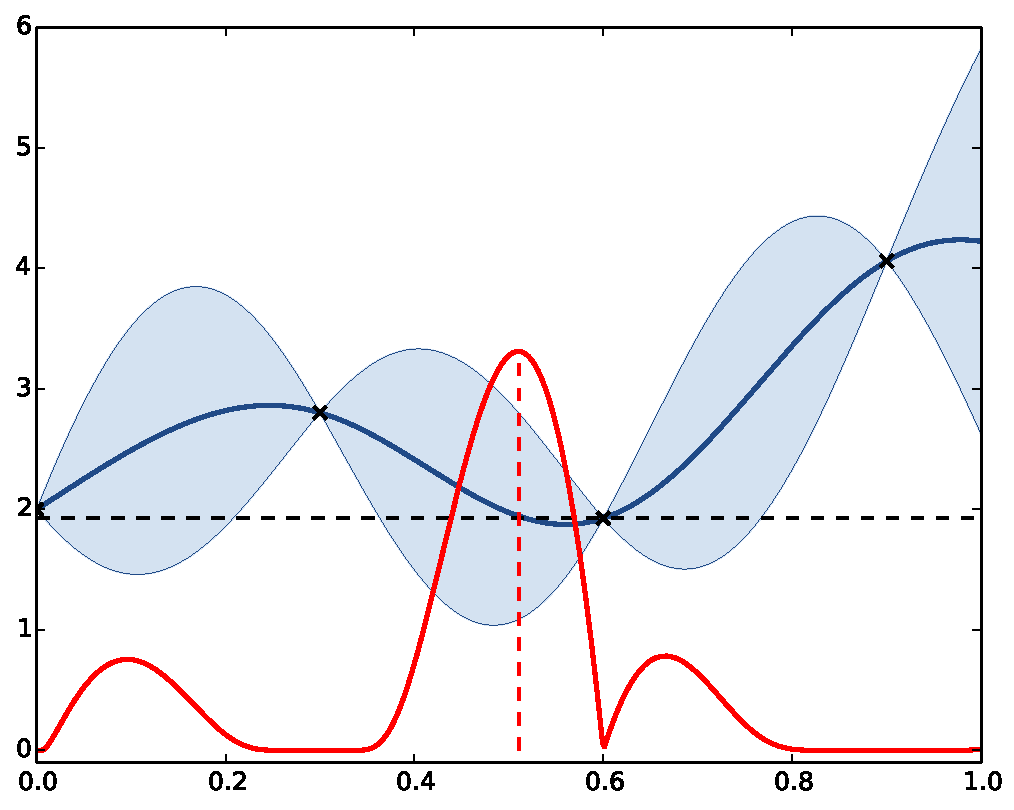
\includegraphics[height=5cm]{figures/python/ego_EI0}
\end{center}
\end{frame}

%%%%%%%%%%%%%%%%%%%%%%%%%%%%%%%%%%%%%%%%%%%%%%%%%%%%%%
\begin{frame}{Expected Improvement}
Let's see how it works... iteration 1
\begin{center}
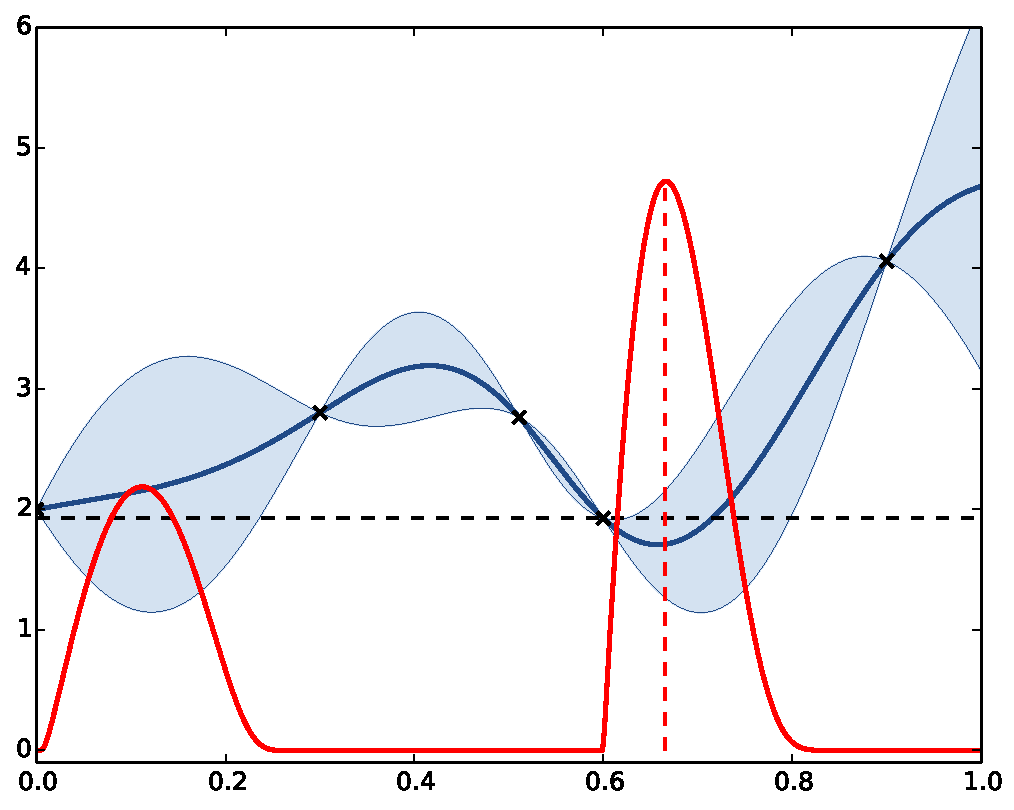
\includegraphics[height=5cm]{figures/python/ego_EI1}
\end{center}
\end{frame}

%%%%%%%%%%%%%%%%%%%%%%%%%%%%%%%%%%%%%%%%%%%%%%%%%%%%%%
\begin{frame}[noframenumbering]{Expected Improvement}
Let's see how it works... iteration 2
\begin{center}
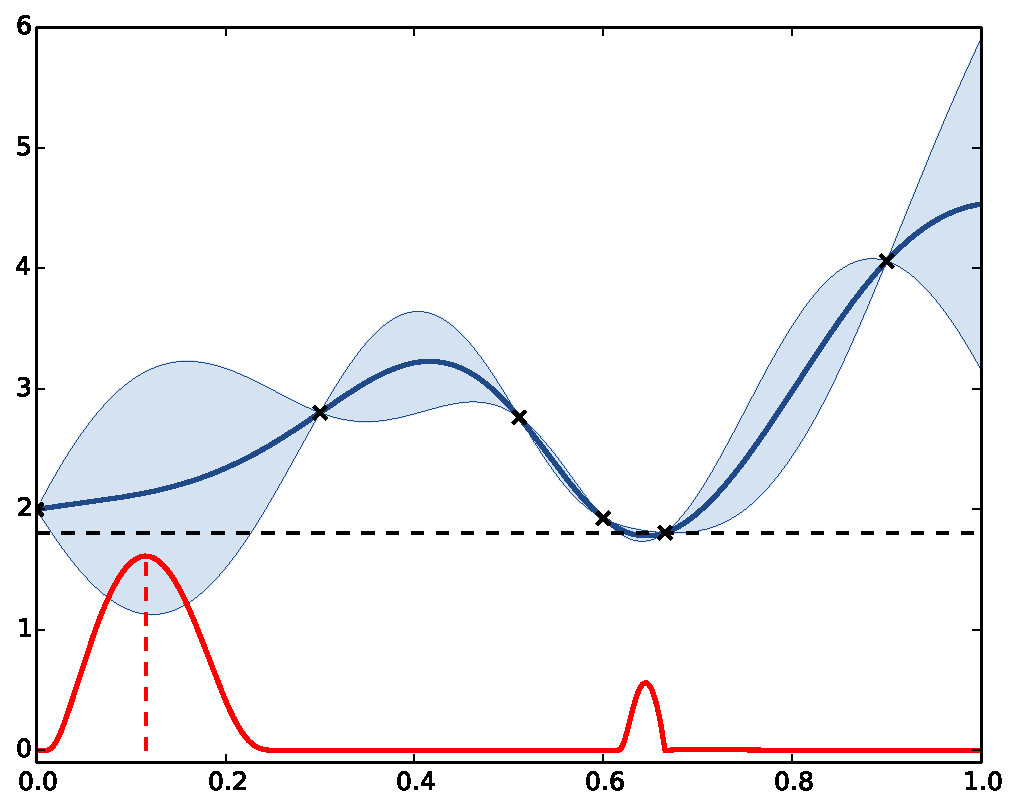
\includegraphics[height=5cm]{figures/python/ego_EI2}
\end{center}
\end{frame}

%%%%%%%%%%%%%%%%%%%%%%%%%%%%%%%%%%%%%%%%%%%%%%%%%%%%%%
\begin{frame}[noframenumbering]{Expected Improvement}
Let's see how it works... iteration 3
\begin{center}
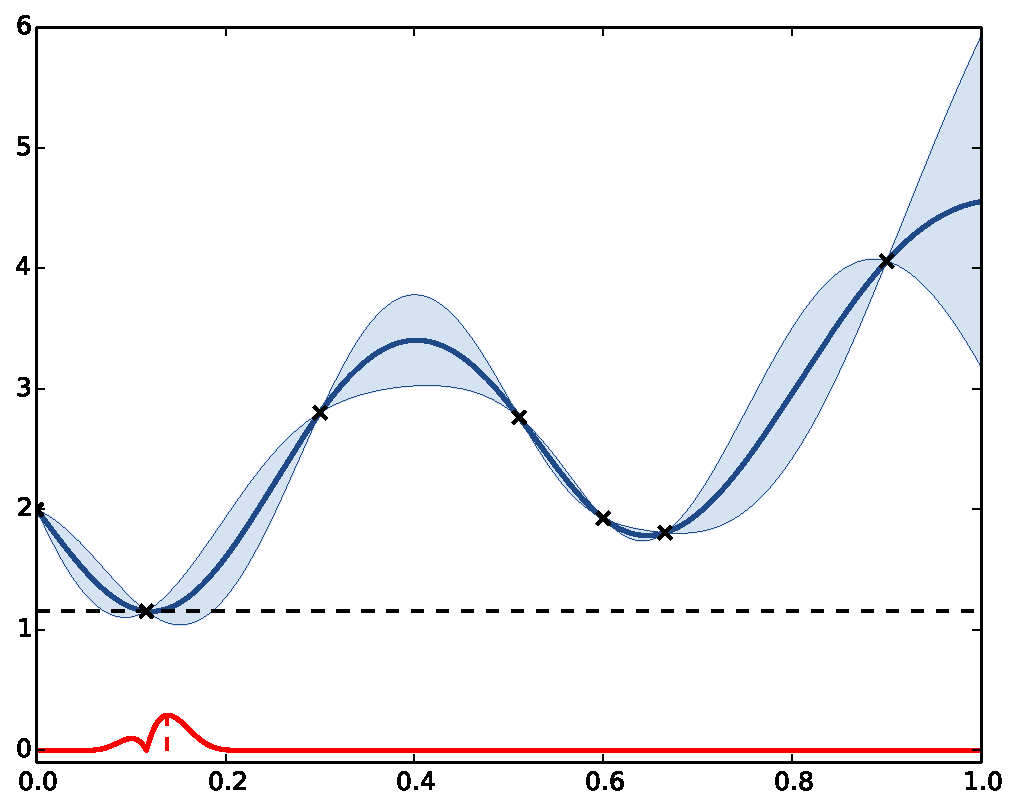
\includegraphics[height=5cm]{figures/python/ego_EI3}
\end{center}
\end{frame}

%%%%%%%%%%%%%%%%%%%%%%%%%%%%%%%%%%%%%%%%%%%%%%%%%%%%%%
\begin{frame}[noframenumbering]{Expected Improvement}
Let's see how it works... iteration 4
\begin{center}
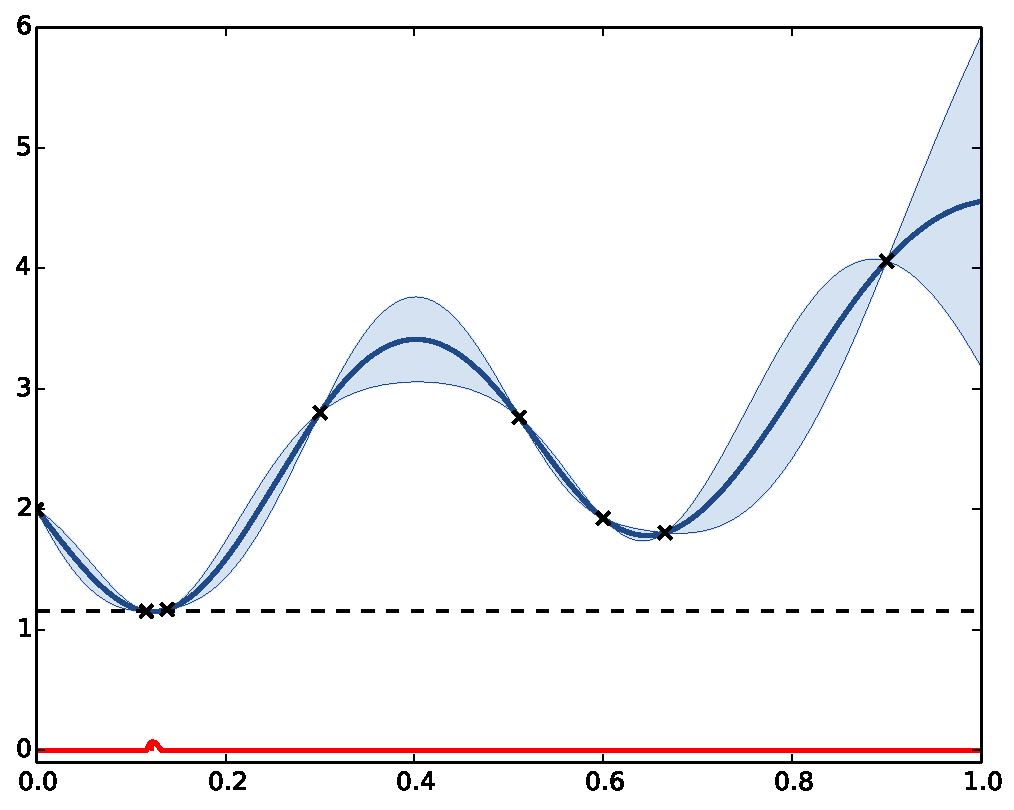
\includegraphics[height=5cm]{figures/python/ego_EI4}
\end{center}
\end{frame}

%%%%%%%%%%%%%%%%%%%%%%%%%%%%%%%%%%%%%%%%%%%%%%%%%%%%%%
\begin{frame}[noframenumbering]{Expected Improvement}
Let's see how it works... iteration 5
\begin{center}
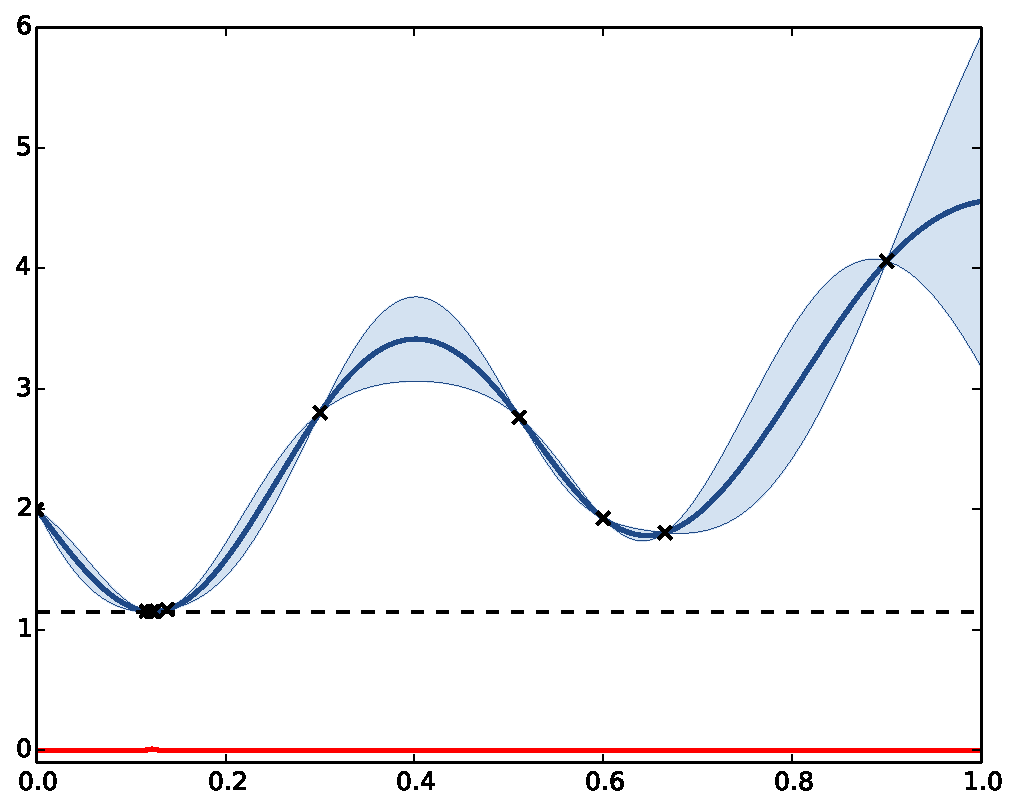
\includegraphics[height=5cm]{figures/python/ego_EI9}
\end{center}
\end{frame}

%%%%%%%%%%%%%%%%%%%%%%%%%%%%%%%%%%%%%%%%%%%%%%%%%%%%%%
\begin{frame}{Expected Improvement}
This algorithm is called \textbf{Efficient Global Optimization} (EGO, Jones et al., 1998):
\begin{enumerate}
	\item make an initial design of experiments $X$ and calculate the associated $F$, $t = \mathtt{length}(F)$
	\item built a GP from $(X,F)$ (max. log-likelihood on $\sigma$ and $\theta_i$'s)
	\item $X_{t+1}= \arg \max_x EI(x)$
	\item calculate $F_{t+1}=f(X_{t+1})$, increment $t$
	\item stop ($t>t^\text{max}$) or go to {\color{blue}2.}
\end{enumerate}
\vspace{5mm}
\begin{itemize}
	\item[+] EGO provides a good trade-off between exploitation and exploration without arbitrary parameters.
	\item[+] It requires few function observations (10 in the example) to get close to optimal regions.
\end{itemize}
%\begin{example}
%From the previous 5 iterations, we obtain $1.44e39$ for the conditioning of the covariance matrix. Eigenvalues are
%$$ (67.70,\  24.86,\  5.13,\  1.68,\  0.45,\  0.16,\  0.01,\  0.00,\  0.00,\ 0.00) $$
%\end{example}
\end{frame}

%%%%%%%%%%%%%%%%%%%%%%%%%%%%%%%%%%%%%%%%%%%%%%%%%%%%%%
%\begin{frame}{}
%\begin{exampleblock}{Illustration for $d=6$ (Hartman)}
%	Illustration in higher dimension
%\begin{center}
%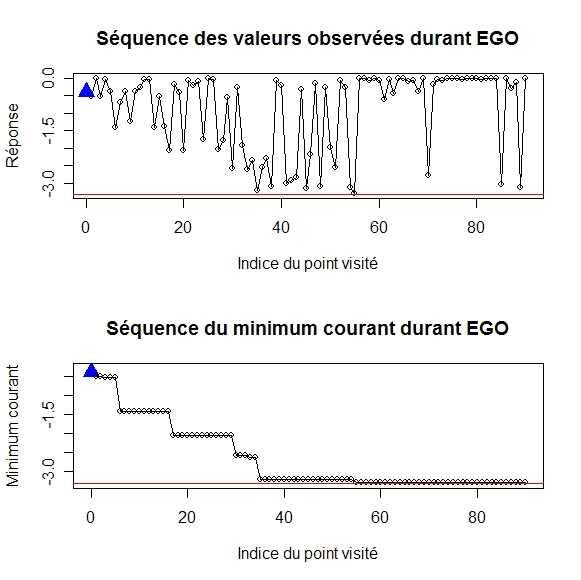
\includegraphics[height=5.5cm]{figures/egoHartman} 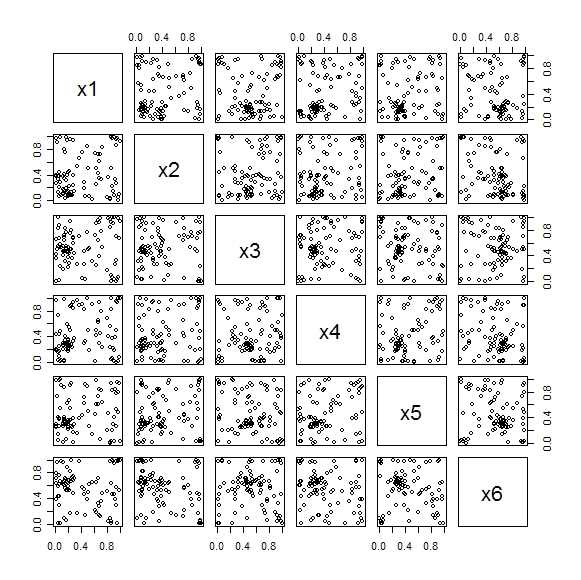
\includegraphics[height=5.5cm]{figures/egoHartman2}
%\end{center}
%\small Source: \textit{DiceOptim}, Roustant, Ginsbourger and Deville, 2009.
%\end{exampleblock}
%\end{frame}

%%%%%%%%%%%%%%%%%%%%%%%%%%%%%%%%%%%%%%%%%%%%%%%%%%%%%%
\begin{frame}{}
\begin{exampleblock}{Example in 5d: surface displacements misfit minimization}
$\Rightarrow$ demo with \texttt{mainInversionPunctualDisplSource.R}\\
!!! normalize the data: WLS has a few very large values, it is always $>0$: make it more gaussian, 
$\mathtt{wls}\_norm = \log(1+\mathtt{wls})$ and all $x$'s and $\mathtt{wls}\_norm$ between 0 and 1.
\begin{minipage}[c]{0.6\textwidth}
\begin{center}
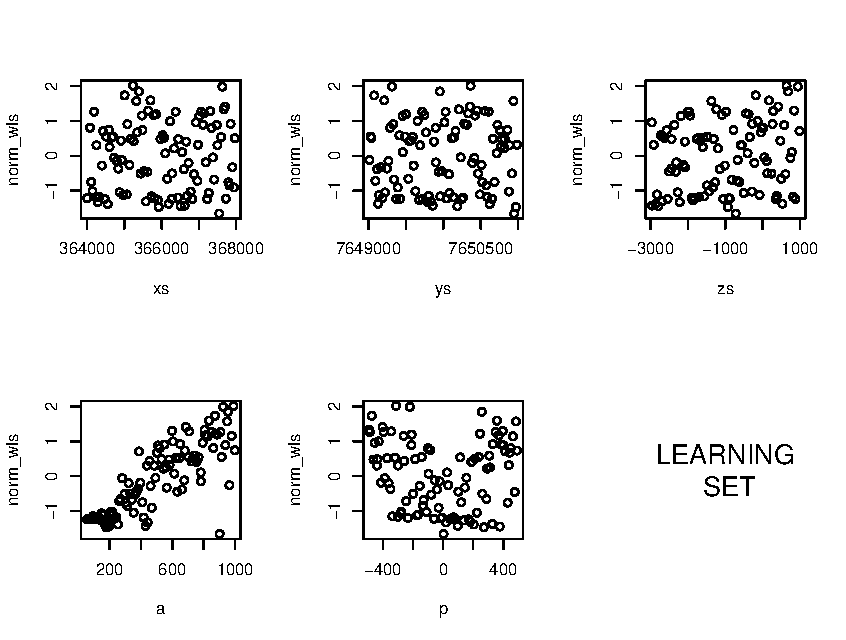
\includegraphics[width=\textwidth]{figures/misfit_learn_set} 
\end{center}
\end{minipage}
\hspace{0.3cm}
\begin{minipage}[c]{0.30\textwidth}
{\small 100 $\{xs,ys,zs,a,p\}$ points chosen through an optimized Latin Hypercube Sampling 
(\texttt{R} libraries \texttt{DiceDesign} or \texttt{lhs}).}\\
\end{minipage}
\end{exampleblock}
\end{frame}

%%%%%%%%%%%%%%%%%%%%%%%%%%%%%%%%%%%%%%%%%%%%%%%%%%%%%%
\begin{frame}{}
\small (demo with \texttt{mainInversionPunctualDisplSource.R}, cont.)
\begin{center}
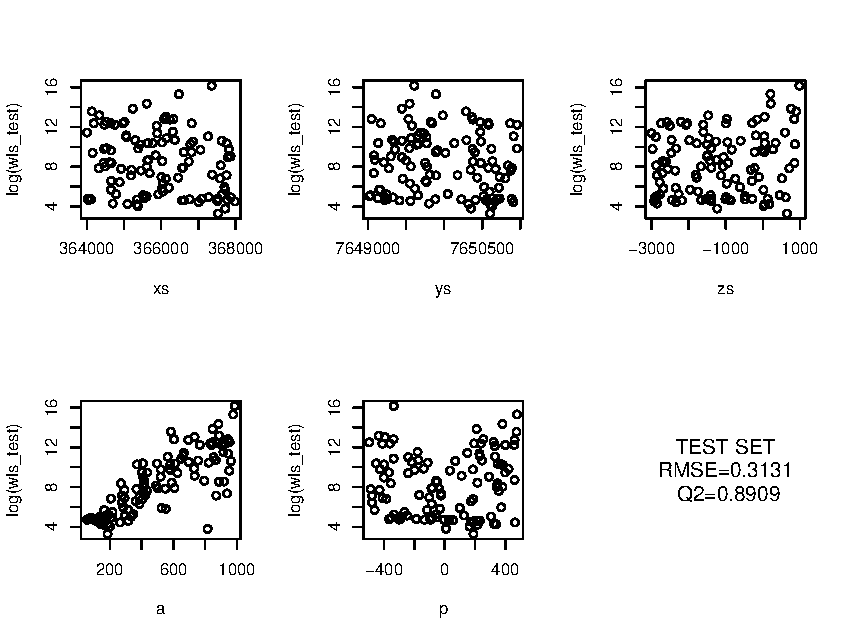
\includegraphics[width=0.7\textwidth]{figures/misfit_test_set} 
\end{center}
{\tiny 110 random $\{xs,ys,zs,a,p\}$ test points.}\\
\end{frame}

%%%%%%%%%%%%%%%%%%%%%%%%%%%%%%%%%%%%%%%%%%%%%%%%%%%%%%
\begin{frame}{}
\small (demo with \texttt{mainInversionPunctualDisplSource.R}, cont.)
\begin{center}
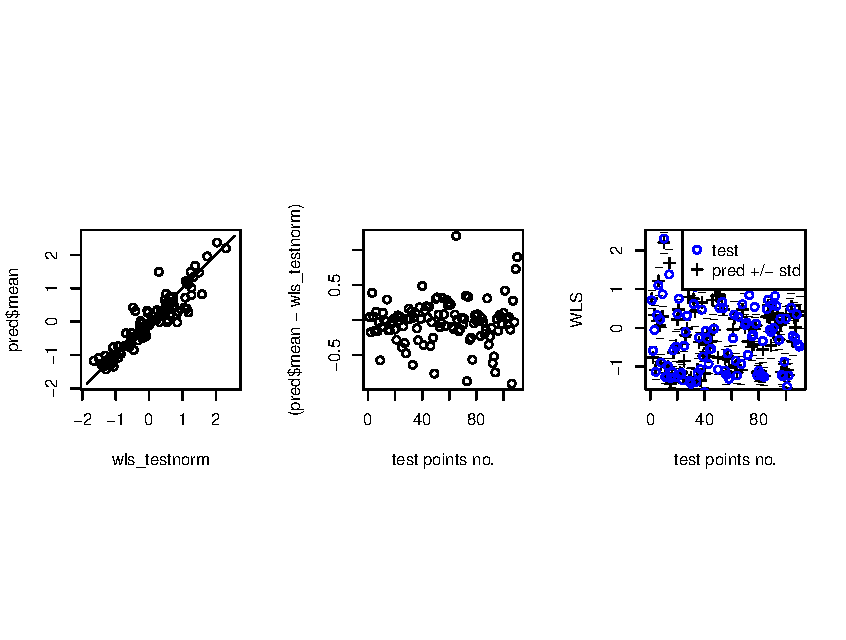
\includegraphics[width=0.9\textwidth]{figures/misfit_test_set_2} 
\end{center}
{\tiny 110 test points.}\\
\end{frame}

%%%%%%%%%%%%%%%%%%%%%%%%%%%%%%%%%%%%%%%%%%%%%%%%%%%%%%
\begin{frame}{}
\small (demo with \texttt{mainInversionPunctualDisplSource.R}, cont.)\\
\small EGO parameters: anisotropic Mat\`ern 5/2 kernel, GP updated (log-likelihood maximized) every 5 added points, BFGS with bounded variables (from \texttt{optim()} function) restarted from random initial points for maximizing log-likelihood and EI.
\begin{minipage}[c]{0.6\textwidth}
\begin{center}
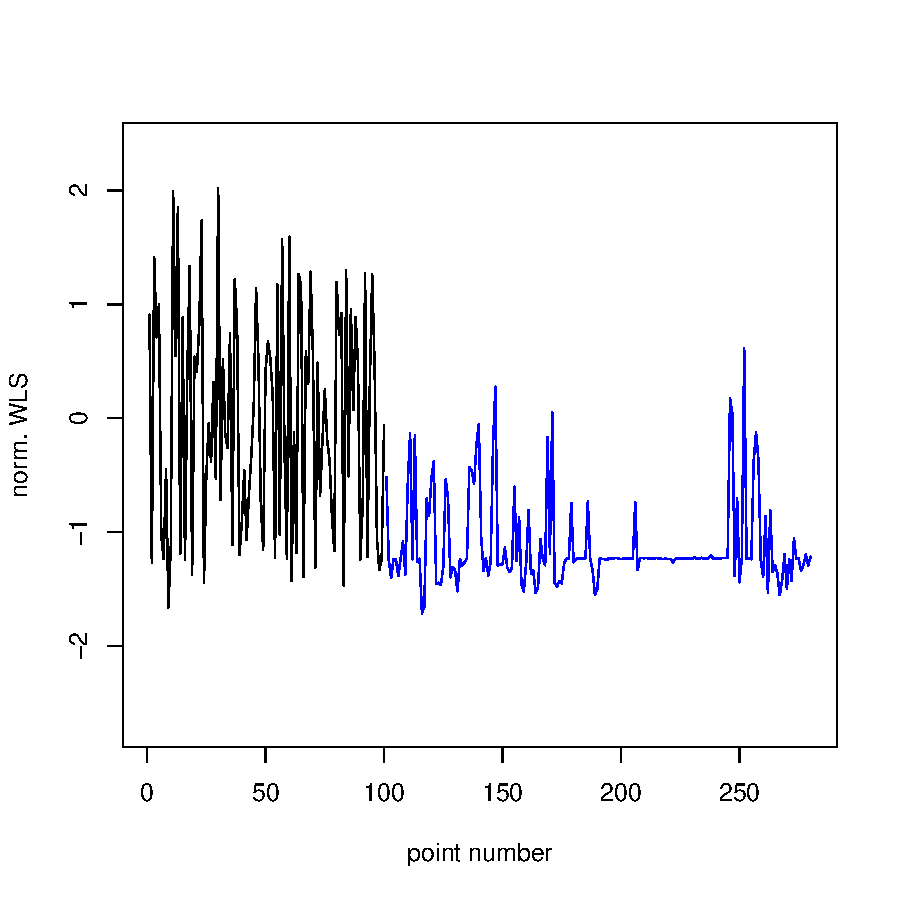
\includegraphics[width=\textwidth]{figures/misfit_EGO_conv} 
\end{center}
\end{minipage}
\hspace{0.3cm}
\begin{minipage}[c]{0.3\textwidth}
Preferential sampling of good regions of $S$, but global therefore sometimes increasing WLS.
Lower bound on $\theta_i$'s increased from 0.08 to 0.1 at $t=250$ ($x_i$'s and $\theta_i$'s
normed between 0 and 1).
\end{minipage}
\end{frame}

%%%%%%%%%%%%%%%%%%%%%%%%%%%%%%%%%%%%%%%%%%%%%%%%%%%%%%
\begin{frame}{}
\small (demo with \texttt{mainInversionPunctualDisplSource.R}, cont.)
\begin{minipage}[c]{0.6\textwidth}
\begin{center}
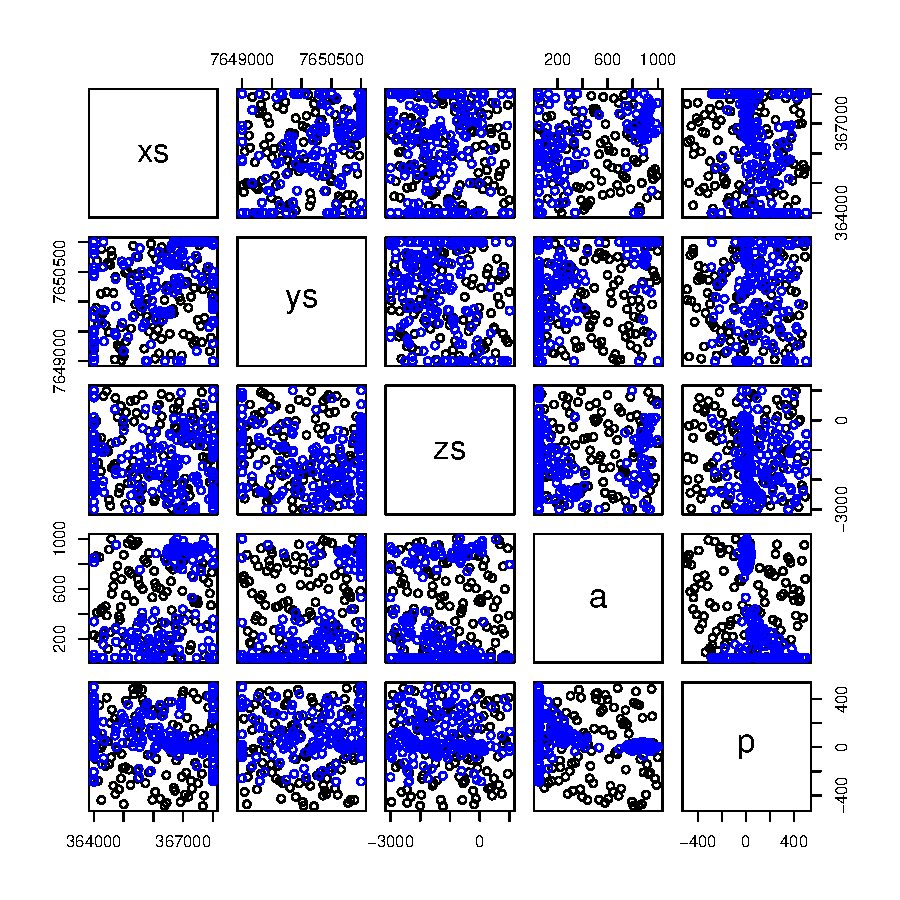
\includegraphics[width=\textwidth]{figures/pairs_X_old_new} 
\end{center}
\end{minipage}
\hspace{0.3cm}
\begin{minipage}[c]{0.3\textwidth}
Black: LHS initial points. \\
Blue: EGO points.\\
\vskip\baselineskip
Note the patterns in new points. Accumulation at lower bound of $a$ and mid interval of $p$ before $t=250$.
\end{minipage}
\end{frame}

%%%%%%%%%%%%%%%%%%%%%%%%%%%%%%%%%%%%%%%%%%%%%%%%%%%%%%
\begin{frame}{}
\small (demo with \texttt{mainInversionPunctualDisplSource.R}, cont.)
\begin{minipage}[c]{0.6\textwidth}
\begin{center}
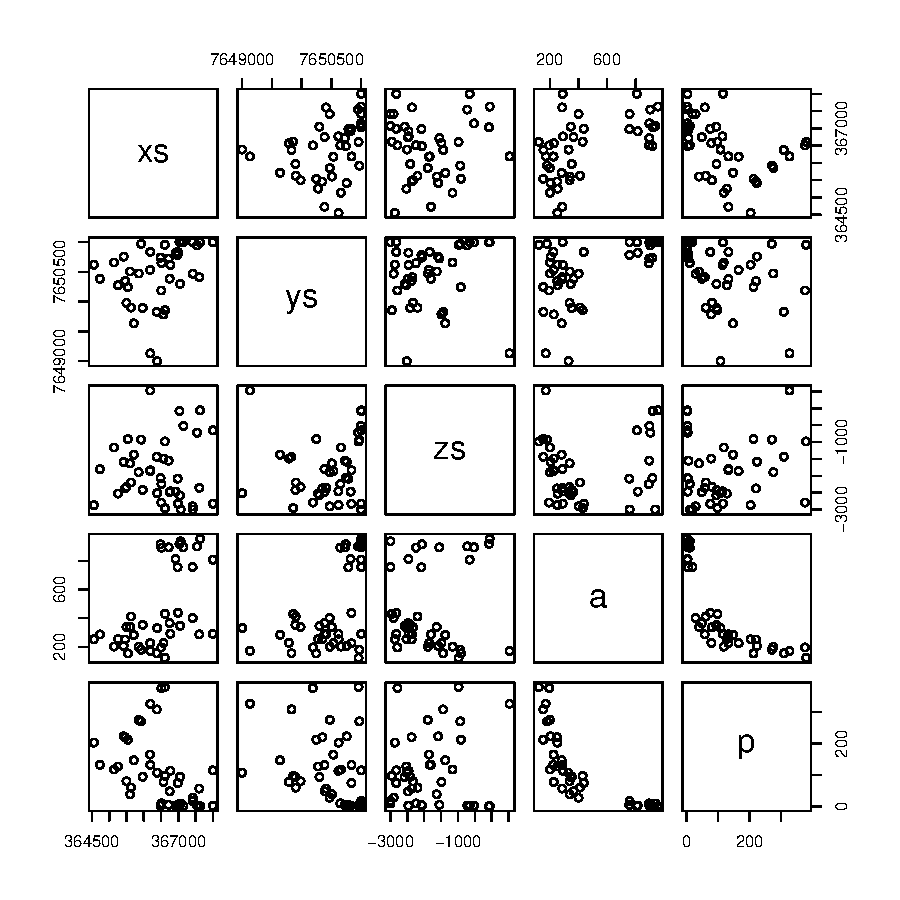
\includegraphics[width=\textwidth]{figures/pairs_X_good_15percent} 
\end{center}
\end{minipage}
\hspace{0.3cm}
\begin{minipage}[c]{0.3\textwidth}
15\% best sampled points. Note the ``function'' for the $(a,p)$ pair, i.e., $a^\star(p^\star)$.
\end{minipage}
\end{frame}

%%%%%%%%%%%%%%%%%%%%%%%%%%%%%%%%%%%%%%%%%%%%%%%%%%%%%%
\begin{frame}{}
\small (demo with \texttt{mainInversionPunctualDisplSource.R}, cont.)
\mbox{ % mbox to avoid linebreak
\begin{minipage}[c]{0.56\textwidth}
\begin{center}
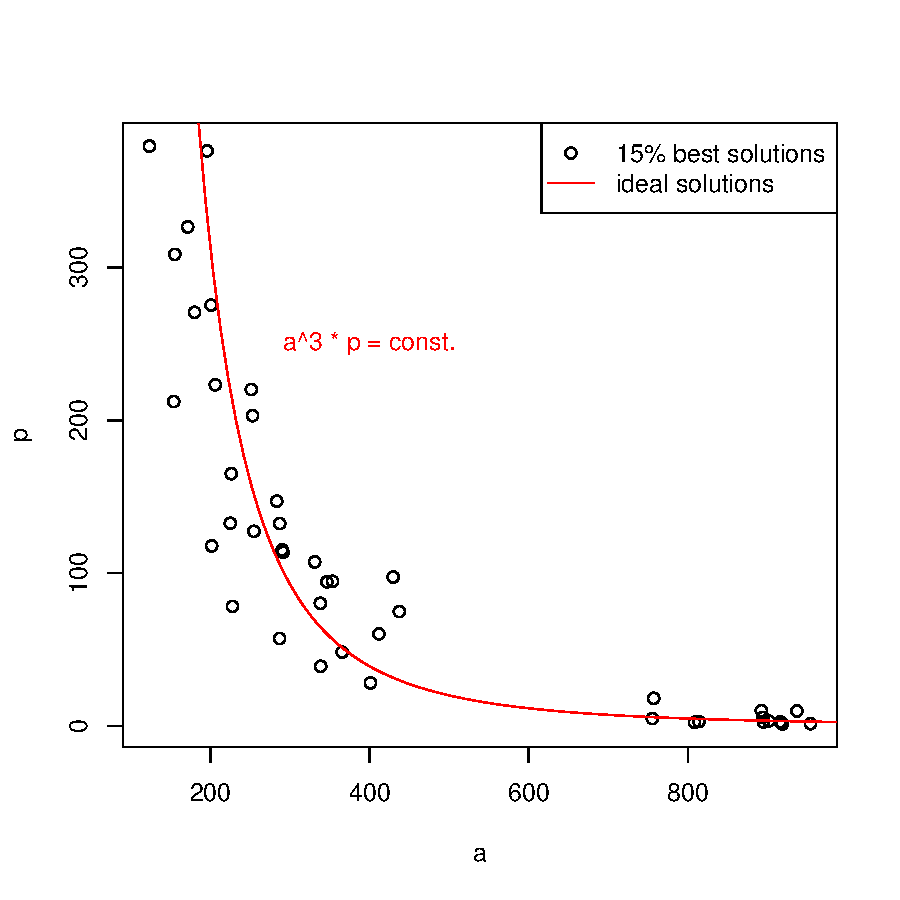
\includegraphics[width=\textwidth]{figures/non_identif_a_p} 
\end{center}
\end{minipage}
\hspace{0.3cm}
\begin{minipage}[c]{0.4\textwidth}
Mogi model only dependency in $a$ and $p$ is through $a^3 \times p$: it is not identifiable. \\
\vskip\baselineskip
EGO tells it by preferential sampling in the valley 
$$a^3 \times p = \text{const.} = {a^\star}^3 \times p^\star$$
\end{minipage}
} % end mbox
Other EGO output: a statistical model of WLS. \\
The last length scales are an indication of the 
sensitivity of WLS to each variable: $a$, $p$ and $zs$ are very sensitive 
($\theta_i$'s small, in $[0.08,0.1]$), $xs$ a little sensitive ($\theta \text{ in } [0.1,2.5]$) 
and $ys$ insensitive ($\theta \approx 3$).
\end{frame}

%%%%%%%%%%%%%%%%%%%%%%%%%%%%%%%%%%%%%%%%%%%%%%%%%%%%%%
\begin{frame}{}
\begin{exampleblock}{Difficulties and challenges with EGO}
\begin{itemize}
\item Standard GPs are limited to $n \approx 1000$ points (covariance matrix inversion).
\item EGO clusters points in good regions, the covariance matrix may become ill-conditionned 
if length scales $\theta_i$ are too large w.r.t. $X$.
\item Although the method perfectly applies to large dimensional spaces ($d>100$), larger $d$ 
may require larger $n$, back 2 lines above.
\item EGO does not converge in the traditional sense: it creates dense samples in the volume of $S$. 
The efficiency comes from the order in which points are sampled.
\end{itemize}
$\Rightarrow$ these are the topics of current research. Let's mention a few extensions next.
\end{exampleblock}
\end{frame}

%%%%%%%%%%%%%%%%%%%%%%%%%%%%%%%%%%%%%%%%%%%%%%%%%%%%%%
\begin{frame}{}
\begin{exampleblock}{EGO continuations}
\begin{itemize}
\item Parallelized EGO: estimate the $EI$ of groups of points, cf. Ginsbourger et al. 
\item Finite budget: $EI$ of a single $x$ is only optimal at the last iteration. Theory of dynamic $EI$, cf. Ginsbourger et al.
\item EGO and bad covariance matrix conditioning: replace points that are close-by by one point and the associated derivatives (cf. M. Osborn, L. Laurent), regularizations (cf. Le Riche et al.)
\item SUR strategies: (Step-wise Uncertainty Reduction), reduce the entropy of the optimum (cf. Vasquez et al.), or the average probability of incursions below $min(F)$ (cf. Picheny).
\end{itemize}
\end{exampleblock}
\end{frame}

%%%%%%%%%%%%%%%%%%%%%%%%%%%%%%%%%%%%%%%%%%%%%%%%%%%%%%
\begin{frame}{}
\begin{exampleblock}{Related problems addressed with GPs}
\begin{itemize}
\item EGO with constraints: $\min_x f(x) \text{ s.t. } g(x) \le 0$, multiply the $EI$ by the probability of constraints satisfaction.
\item GP for target attainment: find the set of $x$ s.t. $f(x) = T$, change the $EI$ into $c(x,x) \times \text{pdf}\left((T-m(x))/sqrt(c(x,x))\right)$, cf. Picheny et al.
\item GP for probability estimation: find $\mathds P (f(x,U)\le T) $ where $U$ is a random vector.
\item GP for multi-objective optimization: $\min_x \{f_1(x), \dots f_m(x)\}$, cf. Binois et al.
\end{itemize}
\end{exampleblock}
\end{frame}

%%%%%%%%%%%%%%%%%%%%%%%%%%%%%%%%%%%%%%%%%%%%%%%%%%%%%%%
%\begin{frame}{}
%One way to improve the conditioning of the covariance matrix is to replace two values that are close-by by one function value and one derivative:
%\begin{center}
%  \begin{tabular}{ccc}
%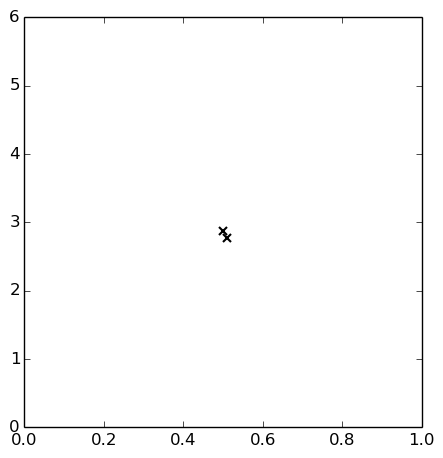
\includegraphics[height=4cm]{figures/python/osborn0} &
%
\includegraphics[height=4cm]{figures/Rightarrow} &
%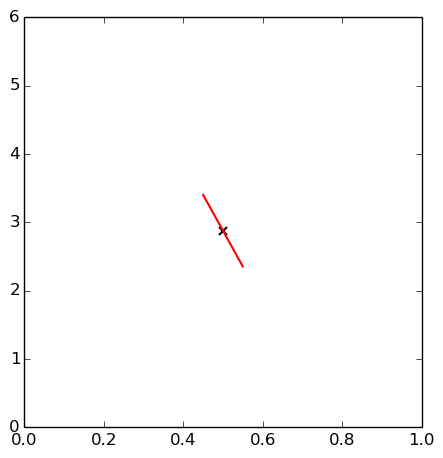
\includegraphics[height=4cm]{figures/python/osborn1} \\
%Cond. = 3842 & & Cond. = 10
%  \end{tabular}
%\end{center}
%This can be generalised to higher orders \alert{$\rightarrow$} Taylor expansion\\
%\small see articles from M. Osborn
%\end{frame}

%%%%%%%%%%%%%%%%%%%%%%%%%%%%%%%%%%%%%%%%%%%%%%%%%%%%%%%
%\begin{frame}{}
%If we know the computational budget in advance, adding new points at the \textbf{best one step ahead location} is not optimal.\\
%\vspace{5mm}
%Some improvements have been made toward this
%\begin{itemize}
%	\item Batch EGO
%	\item Parallelization of the algorithm
%\end{itemize}
%\vspace{5mm}
%\small see works from D. Ginsbourger
%\end{frame}

%%%%%%%%%%%%%%%%%%%%%%%%%%%%%%%%%%%%%%%%%%%%%%%%%%%%%%
%%%%%%%%%%%%%%%%%%%%%%%%%%%%%%%%%%%%%%%%%%%%%%%%%%%%%%
\section[Robust optim.]{Robust optimization}
\subsection{}

%%%%%%%%%%%%%%%%%%%%%%%%%%%%%%%%%%%%%%%%%%%%%%%%%%%%%%%
%\begin{frame}{}
%Robust optimization may mean various things:
%\begin{itemize}
%	\item There is observation noise on the output
%	\item Some input variables $U$ are uncertain
%	\item Model is uncertain, $f(x,U)$
%\end{itemize}
%\vspace{2mm}
%\begin{example}
%\begin{columns}[c]
%\column{3cm}
%	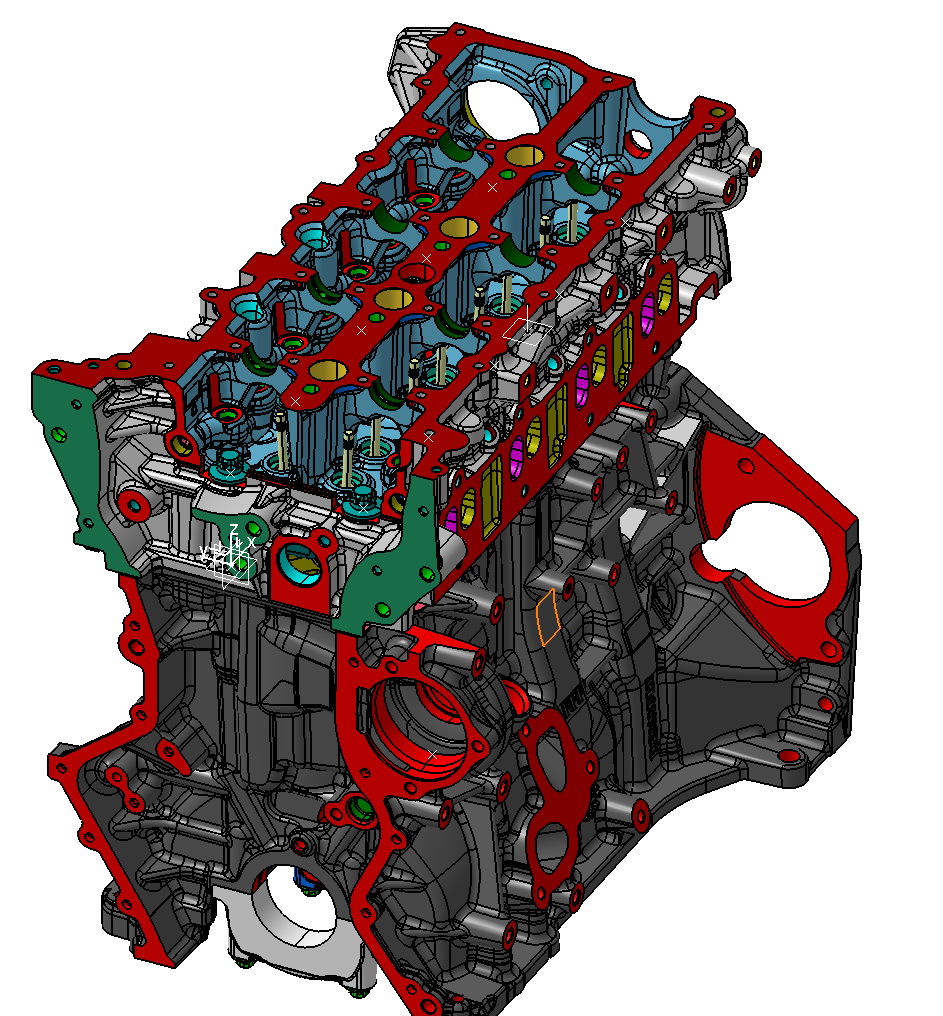
\includegraphics[height=4cm]{figures/RLRrobust}
%\column{5cm}
%	a +/- 1mm dispersion in the manufacturing of a car cylinder head  can degrade its performance (g CO2/km) by -20\% (worst case)\\
%\end{columns}
%\vspace{3mm}
%	\small Source: Talk from R. Le Riche at the Porquerolles Summer School, 2014
%\end{example}
%\end{frame}

%%%%%%%%%%%%%%%%%%%%%%%%%%%%%%%%%%%%%%%%%%%%%%%%%%%%%%
%\begin{frame}{}
% \begin{example}
% Here is a basic example:
% \begin{center}
% 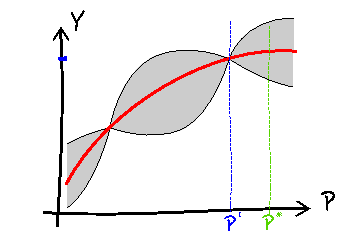
\includegraphics[height=5cm]{figures/optim_rob_a}\\
% Which input is the best?
% \end{center}
% \end{example}
% \end{frame}

%% %%%%%%%%%%%%%%%%%%%%%%%%%%%%%%%%%%%%%%%%%%%%%%%%%%%%%%
%% \begin{frame}[noframenumbering]{}
%\begin{example}
%Here is a basic example:
%\begin{center}
%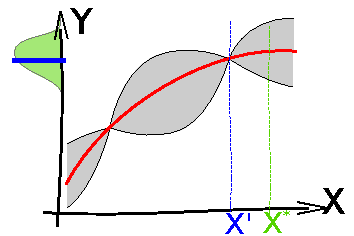
\includegraphics[height=5cm]{figures/optim_rob_b}\\
%Which input is the best?
%\end{center}
%\end{example}
%\end{frame}

%%%%%%%%%%%%%%%%%%%%%%%%%%%%%%%%%%%%%%%%%%%%%%%%%%%%%%%
%\begin{frame}[noframenumbering]{}
%\begin{example}
%A non Gaussian example
%\begin{center}
%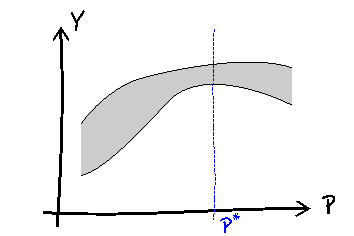
\includegraphics[height=5cm]{figures/optim_rob_c}\\
%In some cases, we may want to optimize the worst case scenario.
%\end{center}
%\end{example}
%\end{frame}

%%%%%%%%%%%%%%%%%%%%%%%%%%%%%%%%%%%%%%%%%%%%%%%%%%%%%%
\begin{frame}{}
Can EGO be adapted when observations are noisy?\\
\vspace{5mm}
First of all, using the current best observation as a minimum does not make much sense...\\
\vspace{5mm}
Some solutions are
\begin{itemize}
	\item[S1] Build a new model that interpolates $m(X)$ at $X$ where $m(X)$ accounts for the noise (non interpolating GP, e.g. with a white noise part in the kernel).
	\item[S2] Include observation noise and replace $\min(F)$ by $\min(m(X))$ in the EI expression
	\item[S3] Similar to 2 but consider an Expected Mean Improvement (V. Picheny).
\end{itemize}
\end{frame}

%%%%%%%%%%%%%%%%%%%%%%%%%%%%%%%%%%%%%%%%%%%%%%%%%%%%%%
\begin{frame}{Solution 1}
iteration 0
\begin{center}
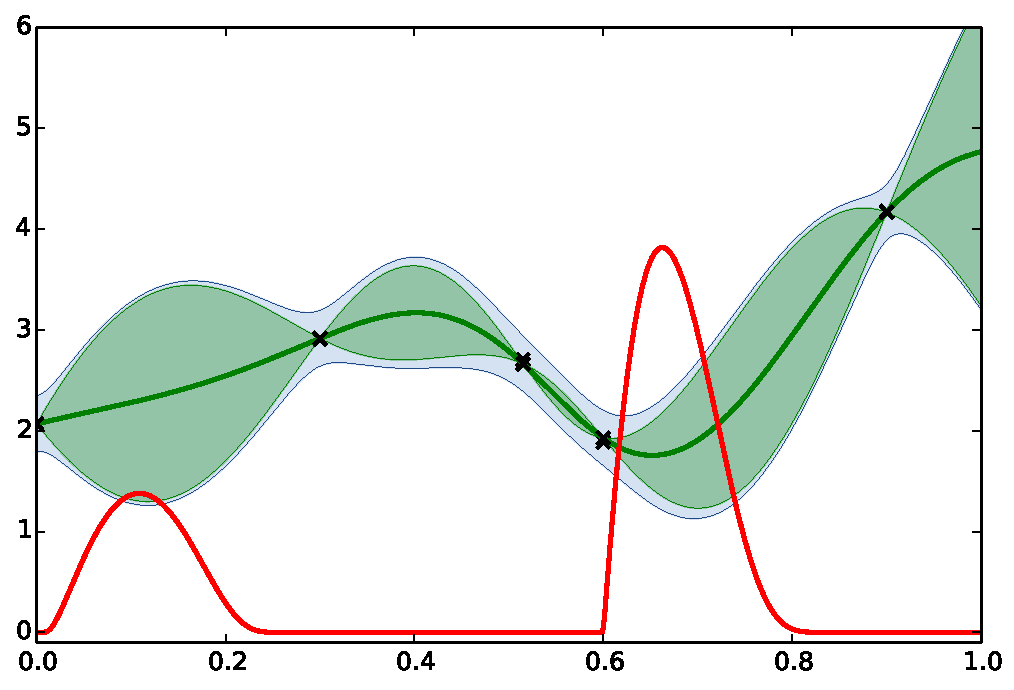
\includegraphics[height=5cm]{figures/python/ego_EI1n0}
\end{center}
\tiny (noisy observations and their denoised versions are both shown as black crosses)\\
\end{frame}

%%%%%%%%%%%%%%%%%%%%%%%%%%%%%%%%%%%%%%%%%%%%%%%%%%%%%%
\begin{frame}[noframenumbering]{Solution 1}
iteration 1
\begin{center}
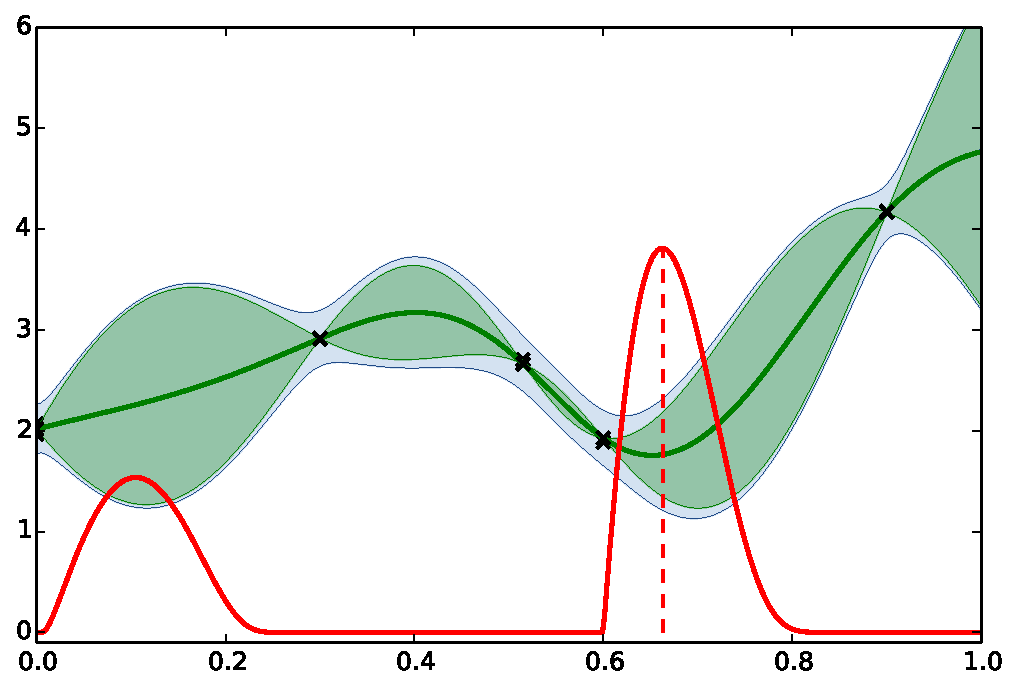
\includegraphics[height=5cm]{figures/python/ego_EI1n1}
\end{center}
\tiny (noisy observations and their denoised versions are both shown as black crosses)\\
\end{frame}

%%%%%%%%%%%%%%%%%%%%%%%%%%%%%%%%%%%%%%%%%%%%%%%%%%%%%%
\begin{frame}[noframenumbering]{Solution 1}
iteration 2
\begin{center}
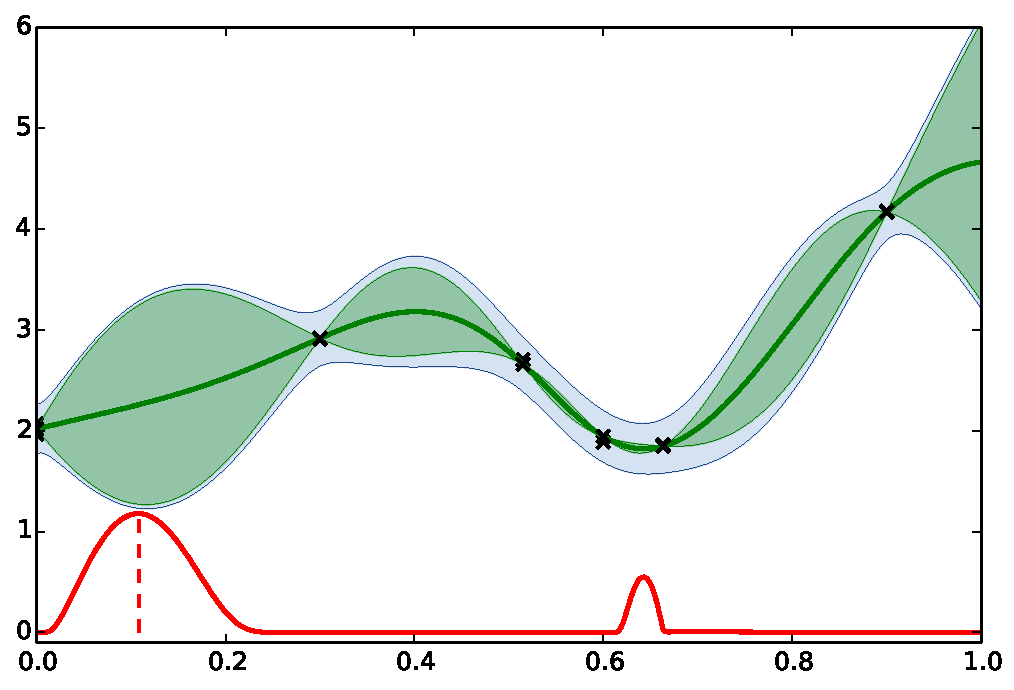
\includegraphics[height=5cm]{figures/python/ego_EI1n2}
\end{center}
\tiny (noisy observations and their denoised versions are both shown as black crosses)\\
\end{frame}

%%%%%%%%%%%%%%%%%%%%%%%%%%%%%%%%%%%%%%%%%%%%%%%%%%%%%%
\begin{frame}[noframenumbering]{Solution 1}
iteration 3
\begin{center}
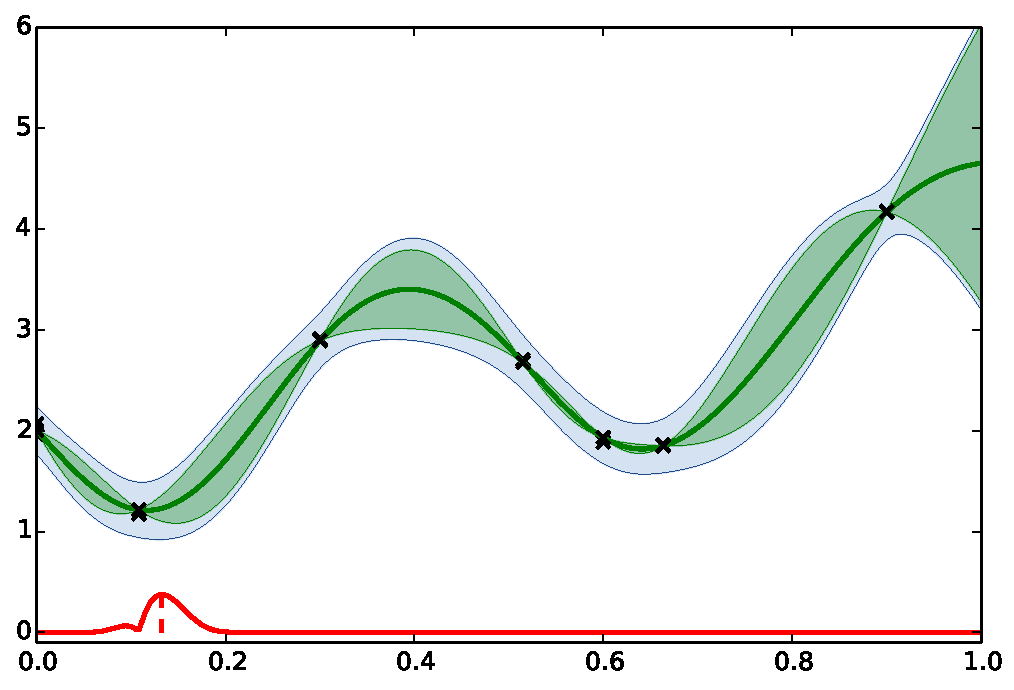
\includegraphics[height=5cm]{figures/python/ego_EI1n3}
\end{center}
\tiny (noisy observations and their denoised versions are both shown as black crosses)\\
\end{frame}

%%%%%%%%%%%%%%%%%%%%%%%%%%%%%%%%%%%%%%%%%%%%%%%%%%%%%%
\begin{frame}[noframenumbering]{Solution 1}
iteration 4
\begin{center}
\includegraphics[height=5cm]{figures/python/ego_EI1n4}
\end{center}
\tiny (noisy observations and their denoised versions are both shown as black crosses)\\
\end{frame}

%%%%%%%%%%%%%%%%%%%%%%%%%%%%%%%%%%%%%%%%%%%%%%%%%%%%%%%
%%%%%%%%%%%%%%%%%%%%%%%%%%%%%%%%%%%%%%%%%%%%%%%%%%%%%%%
%\section[Related problems]{Related problems}
%\subsection{}

%%%%%%%%%%%%%%%%%%%%%%%%%%%%%%%%%%%%%%%%%%%%%%%%%%%%%%%
%\begin{frame}{}
%Some related optimization problems are:
%\begin{itemize}
%	\item calibration problems
%	\item probability computations
%\end{itemize}
%\vspace{8mm}
%Some algorithms with an EGO spirit can be applied:
%\begin{itemize}
% 	\item SUR methods
% \end{itemize}
%\end{frame}

%%%%%%%%%%%%%%%%%%%%%%%%%%%%%%%%%%%%%%%%%%%%%%%%%%%%%%%
%\begin{frame}{}
%We want to find the input(s) such that f(x) = 3.2
%\begin{center}
%\includegraphics[height=5cm]{figures/python/inv}
%\end{center}
%\end{frame}

%%%%%%%%%%%%%%%%%%%%%%%%%%%%%%%%%%%%%%%%%%%%%%%%%%%%%%%
%\begin{frame}[noframenumbering]{}
%iteration 0:
%\begin{center}
%\includegraphics[height=5cm]{figures/python/invproba}
%\end{center}
%\end{frame}

%%%%%%%%%%%%%%%%%%%%%%%%%%%%%%%%%%%%%%%%%%%%%%%%%%%%%%%
%\begin{frame}[noframenumbering]{}
%iteration 1:
%\begin{center}
%\includegraphics[height=5cm]{figures/python/invproba1}
%\end{center}
%\end{frame}

%%%%%%%%%%%%%%%%%%%%%%%%%%%%%%%%%%%%%%%%%%%%%%%%%%%%%%%
%\begin{frame}[noframenumbering]{}
%iteration 2:
%\begin{center}
%\includegraphics[height=5cm]{figures/python/invproba2}
%\end{center}
%\end{frame}

%%%%%%%%%%%%%%%%%%%%%%%%%%%%%%%%%%%%%%%%%%%%%%%%%%%%%%%
%\begin{frame}[noframenumbering]{}
%iteration 3:
%\begin{center}
%\includegraphics[height=5cm]{figures/python/invproba3}
%\end{center}
%\end{frame}

%%%%%%%%%%%%%%%%%%%%%%%%%%%%%%%%%%%%%%%%%%%%%%%%%%%%%%%%%%%%%%%%%%%%%%%%%%%%%%%%%%%%
%%%%%%%%%%%%%%%%%%%%%%%%%%%%%%%%%%%%%%%%%%%%%%%%%%%%%%%%%%%%%%%%%%%%%%%%%%%%%%%%%%%%
\section{Kernel Design}
\subsection{}

%%%%%%%%%%%%%%%%%%%%%%%%%%%%%%%%%%%%%%%%%%%%%%%%%%%%%%
\begin{frame}{}
\structure{Making new from old:}
Many operations can be applied to psd functions while retaining this property
\begin{block}{}
Kernels can be:
\begin{itemize}
  \item Summed together
  \begin{itemize}
    \item On the same space $k(x,y) = k_1(x,y) + k_2(x,y)$
    \item On the tensor space $k(x,y) = k_1(x_1,y_1) + k_2(x_2,y_2)$
  \end{itemize}
  \item Multiplied together
  \begin{itemize}
    \item On the same space $k(x,y) = k_1(x,y) \times k_2(x,y)$
    \item On the tensor space $k(x,y) = k_1(x_1,y_1) \times k_2(x_2,y_2)$
  \end{itemize}
  \item Composed with a function
  \begin{itemize}
    \item $k(x,y) = k_1(f(x),f(y))$
  \end{itemize}
\end{itemize}
\end{block}
\begin{center}
\alert{How can this be useful?}
\end{center}
\end{frame}

% \subsection{Sum of kernels}

%%%%%%%%%%%%%%%%%%%%%%%%%%%%%%%%%%%%%%%%%%%%%%%%%%%%%%
\begin{frame}{Sum of kernels over the same space }
\begin{example}[The Mauna Loa observatory dataset]
This famous dataset compiles the monthly $CO_2$ concentration in Hawaii since 1958.
\begin{center}
\includegraphics[height=4.5cm]{figures/python/CO2-data}
\end{center}
Let's try to predict the concentration for the next 20 years.
\end{example}
\end{frame}

%%%%%%%%%%%%%%%%%%%%%%%%%%%%%%%%%%%%%%%%%%%%%%%%%%%%%%
\begin{frame}{Sum of kernels over the same space }
We first consider a squared-exponential kernel:
$$ \displaystyle k_{se}(x,y) = \sigma^2\exp \left(-\frac{(x-y)^2}{\theta^2} \right)$$
\begin{center}
\includegraphics[height=3.7cm]{figures/python/CO2-rbfa} \quad \includegraphics[height=3.7cm]{figures/python/CO2-rbfb}
\end{center}
\begin{block}{}
\centering
\alert{The results are terrible!}
\end{block}
\end{frame}

%%%%%%%%%%%%%%%%%%%%%%%%%%%%%%%%%%%%%%%%%%%%%%%%%%%%%%
\begin{frame}{Sum of kernels over the same space }
What happen if we sum both kernels?
\begin{equation*}
k(x,y) = k_{se1}(x,y) + k_{se2}(x,y)
\end{equation*}
\pause
\begin{center}
\vspace{-8mm} \includegraphics[height=4.5cm]{figures/python/CO2-rbfab}
\end{center}
%\vspace{1mm}
\begin{block}{}
\centering
\alert{The model is drastically improved!}
\end{block}
\end{frame}

%%%%%%%%%%%%%%%%%%%%%%%%%%%%%%%%%%%%%%%%%%%%%%%%%%%%%%
\begin{frame}{Sum of kernels over the same space }
We can try the following kernel:
\begin{equation*}
k(x,y) = \sigma_0^2  x^2 y^2 + k_{se1}(x,y) + k_{se2}(x,y) + k_{per}(x,y)
\end{equation*}
\pause
\begin{center}
\vspace{-8mm}  \includegraphics[height=4.5cm]{figures/python/CO2-rbfabpq}
\end{center}
\begin{block}{}
\centering
\alert{Once again, the model is significantly improved.}
\end{block}
\end{frame}


%%%%%%%%%%%%%%%%%%%%%%%%%%%%%%%%%%%%%%%%%%%%%%%%%%%%%%
\begin{frame}{Sum of kernels over tensor space}
\begin{block}{Property}
\begin{equation*}
k(x,y) = k_1(x_1,y_1) +  k_2(x_2,y_2)
\end{equation*}
is valid covariance structure.\\
\begin{columns}[c]
\begin{column}{3cm}
\includegraphics[width=3cm]{figures/python/newfromold-sum2-k1}
\end{column}
\begin{column}{2mm}
$+$
\end{column}
\begin{column}{3cm}
\includegraphics[width=3cm]{figures/python/newfromold-sum2-k2}
\end{column}
\begin{column}{2mm}
$=$
\end{column}
\begin{column}{3cm}
\includegraphics[width=3cm]{figures/python/newfromold-sum2-k12}
\end{column}
\end{columns}
\vspace{4mm}
\end{block}
\structure{Remark:}
From a GP point of view, $k$ is the kernel of
$$Z(x) = Z_1(x_1) + Z_2(x_2)$$
\end{frame}

%%%%%%%%%%%%%%%%%%%%%%%%%%%%%%%%%%%%%%%%%%%%%%%%%%%%%%
\begin{frame}{Sum of kernels over tensor space}
We can have a look at a few sample paths from $Z$:
\begin{center}
\includegraphics[width=3.5cm]{figures/python/newfromold-sum2-traj124} \includegraphics[width=3.5cm]{figures/python/newfromold-sum2-traj121} \includegraphics[width=3.5cm]{figures/python/newfromold-sum2-traj123} % \includegraphics[width=3.5cm]{figures/newfromold-sum2-traj122}
\end{center}
\qquad \alert{$\Rightarrow$ They are additive (up to a modification)}\\ \ \\
Tensor Additive kernels are very useful for
\begin{itemize}
  \item Approximating additive functions
  \item Building models over high dimensional inputs spaces
\end{itemize}
\end{frame}

%%%%%%%%%%%%%%%%%%%%%%%%%%%%%%%%%%%%%%%%%%%%%%%%%%%%%%
\begin{frame}{Product over the same space}
\begin{block}{Property}
\begin{equation*}
k(x,y) = k_1(x,y) \times  k_2(x,y)
\end{equation*}
is valid covariance structure.
\end{block}
%\vspace{10mm}
\begin{example}
We consider the product of a squared exponential with a cosine:
\begin{columns}[c]
\begin{column}{3cm}
\includegraphics[width=3cm]{figures/python/newfromold-pa.pdf}
\end{column}
\begin{column}{2mm}
$\times$
\end{column}
\begin{column}{3cm}
\includegraphics[width=3cm]{figures/python/newfromold-pb.pdf}
\end{column}
\begin{column}{2mm}
$=$
\end{column}
\begin{column}{3cm}
\includegraphics[width=3cm]{figures/python/newfromold-pab1.pdf}
\end{column}
\end{columns}
\vspace{5mm}
\end{example}
\end{frame}

%%%%%%%%%%%%%%%%%%%%%%%%%%%%%%%%%%%%%%%%%%%%%%%%%%%%%%
\begin{frame}{Product over the tensor space}
\begin{block}{Property}
\begin{equation*}
k(x,y) = k_1(x_1,y_1) \times k_2(x_2,y_2)
\end{equation*}
is valid covariance structure.
\end{block}
%\vspace{10mm}
\begin{example}
We multiply 2 squared exponential kernel
\begin{columns}[c]
\begin{column}{3cm}
\includegraphics[width=3cm]{figures/python/newfromold-sum2-k1}
\end{column}
\begin{column}{2mm}
$\times $
\end{column}
\begin{column}{3cm}
\includegraphics[width=3cm]{figures/python/newfromold-sum2-k2}
\end{column}
\begin{column}{2mm}
$=$
\end{column}
\begin{column}{3cm}
\includegraphics[width=3cm]{figures/python/newfromold-prod2-k12}
\end{column}
\end{columns}
\vspace{5mm}
Calculation shows this is the usual 2D squared exponential kernel.
\end{example}
\end{frame}

% \subsection{Composition with a function}

%%%%%%%%%%%%%%%%%%%%%%%%%%%%%%%%%%%%%%%%%%%%%%%%%%%%%%
\begin{frame}{Composition with a function}
\begin{block}{Property}
Let $k_1$ be a kernel over $D_1 \times D_1$ and $f$ be an arbitrary function $D \rightarrow D_1$, then
\begin{equation*}
k(x,y) = k_1(f(x),f(y))
\end{equation*}
is a kernel over $D \times D $.\\
\small
\textbf{proof}\\
\begin{equation*}
\sum \sum a_i  a_j k(x_i,x_j) = \sum \sum a_i a_j k_1(\underbrace{f(x_i)}_{y_i},\underbrace{f(x_j)}_{y_j}) \geq 0
\end{equation*}
\end{block}
\vspace{5mm}
\structure{Remarks:}
\begin{itemize}
\item $k$ corresponds to the covariance of $Z(x) = Z_1(f(x))$
\item This can be seen as a (non-linear) rescaling of the input space
\end{itemize}
\end{frame}

%%%%%%%%%%%%%%%%%%%%%%%%%%%%%%%%%%%%%%%%%%%%%%%%%%%%%%
\begin{frame}{}
\begin{example}
We consider $f(x) = \frac1x$ and a Mat\'ern 3/2 kernel $k_1(x,y) = (1 + |x-y|) e^{-|x-y|}$.\\ \vspace{5mm}
\textbf{We obtain:}
\begin{columns}[c]
\begin{column}{5cm}
\begin{center}
Kernel
\includegraphics[width=4cm]{figures/python/newfromold-compfunc-k}
\end{center}
\end{column}
\begin{column}{5cm}
\begin{center}
Sample paths
\includegraphics[width=4cm]{figures/python/newfromold-compfunc-traj}
\end{center}
\end{column}
\end{columns}
\end{example}
\end{frame}

%%%%%%%%%%%%%%%%%%%%%%%%%%%%%%%%%%%%%%%%%%%%%%%%%%%%%%
\begin{frame}{}
\structure{All these transformations can be combined!}
\begin{example}
$k(x,y) = f(x)f(y)k_1(x,y)$ is a valid kernel.\\
\vspace{0.5cm}
This can be illustrated with $f(x) = \frac1x$ and $k_1(x,y) = (1 + |x-y|) e^{-|x-y|}$:\\
\begin{columns}[c]
\begin{column}{5cm}
\begin{center}
Kernel
\includegraphics[width=4cm]{figures/python/newfromold-prodfunc-k}
\end{center}
\end{column}
\begin{column}{5cm}
\begin{center}
Sample paths
\includegraphics[width=4cm]{figures/python/newfromold-prodfunc-traj}
\end{center}
\end{column}
\end{columns}
\end{example}
\end{frame}


%%%%%%%%%%%%%%%%%%%%%%%%%%%%%%%%%%%%%%%%%%%%%%%%%%%%%%
\begin{frame}{}
\begin{exampleblock}{Example}
\begin{center}
\includegraphics[height=4cm]{figures/piton_fournaise_5dike_intrusions_98_00} 
\end{center}
\end{exampleblock}
\alert{$\Rightarrow$ R demo}
\end{frame}


%%%%%%%%%%%%%%%%%%%%%%%%%%%%%%%%%%%%%%%%%%%%%%%%%%%%%%
\begin{frame}{Other kernel design methods}
There are two other popular methods for kernel design:
\begin{itemize}
    \item Bochner Theorem\\
There is an equivalence between positive measures and stationnary positive definite functions. 
    \item Linear operators\\
If the function to approximate has particular properties that can be obtained via a linear transform, it is possible to build a GP with the wanted properties. For example, one can build symmetric GPs or GPs with integral equal to zero.
\end{itemize}
\end{frame}


%%%%%%%%%%%%%%%%%%%%%%%%%%%%%%%%%%%%%%%%%%%%%%%%%%%%%%%%%%%%%%%%%%%%%%%%%%%%%%%
%%%%%%%%%%%%%%%%%%%%%%%%%%%%%%%%%%%%%%%%%%%%%%%%%%%%%%%%%%%%%%%%%%%%%%%%%%%%%%%
%%%%%%%%%%%%%%%%%%%%%%%%%%%%%%%%%%%%%%%%%%%%%%%%%%%%%%%%%%%%%%%%%%%%%%%%%%%%%%%
%%%%%%%%%%%%%%%%%%%%%%%%%%%%%%%%%%%%%%%%%%%%%%%%%%%%%%%%%%%%%%%%%%%%%%%%%%%%%%%
\end{document}
